\documentclass[
    % Specify hyperref options
    colorlinks=true,        % Colour all links
    linkcolor=black,          % Cross-references in red
    anchorcolor=black,      % Keep anchors black
    citecolor=black,         % In-text-referencs in blue
    urlcolor=black,          % DOIs and URLs are in blue
    bookmarks=true,         % Generate bookmarks for PDF readers
    bookmarksopen=false,    % Expand all bookmarks as default
    bookmarksnumbered=true,  % Keep section number in bookmarks
    % Specify xcolor options
    dvipsnames
]{MAE}

\title{Your Thesis Title May Span for a Maximum of Three Lines on the Cover Page}
\subtitle{While Your Subtitle Can Occupy at Most Two Lines Such as This}
\candidate{Firstname Lastname}
\semester{Spring 2021}

\usepackage{MAE}

\begin{document}
\makeMAEtitle

\chapter*{Popular Abstract}
\label{Ab.0}

\noindent Preparing youth for life-long success with numeracy, literacy and science capability has been the core mission for all schooling systems. The post-financial crises and post-COVID era, in addition, imposed increasing demand for financial literacy on school leavers. Although financial education programs were generally reported as effective in promoting learners' financial literacy outcome, paradoxical results of non-findings or even negative findings were not unheard of. Any claim that education efforts did not matter, or even harmful, for learners' development deserves immediate attention because if school were committing something wrong, school leaders and policy makers would want to know what, which and where the problems were so that harmful practices can be reverted into good pedagogy. Alternatively, it could instead be the instrument some researchers employed that led to such underwhelming results. A closer examination of how school effectiveness is measured would also promote methodology practices and the resultant policy advice. Using 2018 PISA financial literacy data, this study examined how students' financial literacy scores changed systematically as educational efforts, parental involvement, school safety as well as resource allocation varied. Analyses showed that all four aspects of school climate mattered greatly in explaining differences in students' financial literacy scores. Negative results reported by some papers were likely the results of certain design choices. School financial education should definitely not be withdrawn but more carefully designed with increase emphases on students' financial problem-solving skills in addition to knowledge and confidence training.


\section*{Acknowledgements}

Maecenas vel maximus erat. Vestibulum ac ornare neque. Integer vestibulum elit sem, ac varius turpis dapibus sed. Nulla erat neque, consectetur nec urna pretium, finibus elementum urna. Donec id hendrerit sem. Cras et arcu nunc. Nam dictum lacus vitae lorem luctus ultricies. Suspendisse varius velit quis imperdiet rhoncus. Quisque ut placerat nulla. Cras ut tortor mattis, finibus nisi non, sollicitudin purus. Vestibulum dolor elit, accumsan id ligula eget, lobortis malesuada lorem. Aenean vel maximus justo.

Proin pretium venenatis tortor, id varius turpis semper non. Sed non elit eget purus cursus ultrices et sit amet diam. Morbi vestibulum tortor magna, sed placerat justo condimentum ac. Morbi leo magna, pharetra in neque eget, fringilla aliquam elit. Duis at ultrices ligula. Suspendisse ac ligula in tortor condimentum feugiat. Etiam ut ligula id sapien efficitur malesuada. Sed nec sagittis nisi, nec auctor dolor. Proin viverra feugiat gravida. Quisque venenatis a risus non venenatis.

In hac habitasse platea dictumst. Sed finibus laoreet quam a mollis. Phasellus turpis est, convallis ut enim ut, aliquet sodales metus. Mauris porta lectus et dolor vehicula semper. Proin volutpat feugiat nibh ut blandit. Morbi mollis nunc et leo ultrices, id posuere ipsum semper. Quisque auctor egestas dignissim. Nunc molestie nulla ac enim tincidunt, non scelerisque enim hendrerit. Nulla bibendum dolor eget tellus porttitor, at auctor velit accumsan. Donec at volutpat eros, eu varius turpis. Phasellus a pellentesque enim.

Aenean id tellus eu ex tempor finibus. Vestibulum ante ipsum primis in faucibus orci luctus et ultrices posuere cubilia curae; Suspendisse gravida volutpat lacinia. Integer imperdiet sagittis suscipit. Aliquam vitae tristique ante. Morbi diam lorem, efficitur sit amet luctus eu, placerat eget neque. Sed quis pretium metus, in bibendum dui. Duis feugiat, justo ut convallis gravida, diam ipsum mattis massa, vitae mollis risus ligula ut quam. Ut feugiat dignissim quam in auctor. Nunc rutrum nec est at iaculis.


% Insert a blank page if preambles end on an odd page so Page 1 starts right.
\cleardoublepage

% Use arabic numbers for main pages
\pagenumbering{arabic}

\section{\MAEtitle: \MAEsubtitle}

% Never start your introduction with a heading "Introduction".

%//mark Broad motivation

\subsection{An Atlas of Financial Illiteracy}

Repeated economic crises in recent memory have exposed the harsh consequences of financial \emph{illiteracy} shared by high proportions of the general population. Low financial literacy was directly linked with negative credit behaviours such as high amount of credit card debt \parencite{norvilitis:2010}, high costs of borrowing \parencite{huston:2012, pak:2018}, poor mortgage choices \parencite{cox:2015} and subsequent delinquency and home foreclosure \parencite{agarwal:2015a, gerardi:2010}. Poor financial decisions made early in life can have profound long-term economic and societal impacts \parencite{montoya:2013} such as forgoing medical care \parencite{lusardi:2015}, mental health crises \parencite{stone:2018} and geronto-poverty resultant from insufficient retirement provision \parencite{lusardi:2007, lusardi:2008}. Borrowers' collective misjudgement on mortgage risks kicked start the subprime crises and in combination with Wall Street greed and laissez faire regulatory attitudes that eventually triggered the avalanche of 2008 financial crisis, the first domino of world-changing events whose impact continues reshaping global economics and geopolitics landscape.

Even more concerning is the pervasive global distribution of financial illiteracy. Deficiencies in financial capability had been observed not only in emerging economies \parencite{karakurumozdemir:2019} such as Colombia \parencite{caoalvira:2020}, Mexico \parencite{arceogomez:2017, bohm:2021}, India \parencite{agarwal:2015b, kiliyanni:2016, utkarsh:2020}, Indonesia \parencite{cole:2009, khoirunnisaa:2020}, Turkey \parencite{akbenselcuk:2014}, and Eastern European countries \parencite{belas:2016, opletalova:2015, reiter:2020} but also in advanced economies such as Australia \parencite{ali:2014, taylor:2013, thomson:2017}, Canada \parencite{boisclair:2017}, Germany \parencite{bucherkoenen:2017, erner:2016}, Austria \parencite{silgoner:2015}, the UK \parencite{barnard:2021} and the USA \parencite{breitbach:2016, gale:2012, lusardi:2010}. International comparisons also reported low financial literacy in many Asian countries \parencite{yoshino:2015} and member states of the Organisation for Economic Co-operation and Development (OECD) \parencite{cupak:2018a, lusardi:2015a}, particularly amongst the young \parencite{debeckker:2019}, females, lower educated \parencite{klapper:2019} and somewhat surprising, inhabitants of countries with more generous social security systems \parencite{jappelli:2010}.

\subsection{Financial Literacy as a Necessity}

One major reason behind the escalating interests in citizens' financial literacy can be attributed to the policy adjustment taking place in the past two decades. The neo-liberal ideology of reducing government involvement in the economy had crowded out societal care such as pension, health and education from the collective via the state to the individuals \parencite{gilbert:2002}. In a post-financialisation world \parencite{krippner:2005}, the primary goal of political economy has shifted from the redistribution of wealth to the incorporation of individuals within the mainstream financial architecture \parencite{regan:2003}. The succession of the asset-based welfare system to the income-based model \parencite{finlayson:2009}, however, was by no means unique to the Anglosphere. The Hartz reforms of 2003/04, according to \textcite{seeleibkaiser:2016}, had significantly altered Germany's post-war social welfare arrangement, leading \textcite{ferragina:2015} to re-classify Germany from a conservative welfare into a liberal welfare state comparable to the United Kingdom. Although a detailed account of the history, politics and moral philosophy of social welfare reforms is beyond the scope of this project, this background information does confirm financial literacy as a social necessity independent of one's believes or preference.

Strengthening citizen's financial literacy also generates substantial social returns. The latest U.S. Department of Justice statistics showed a total loss of near 3.25 billion dollars to financial fraud in 2017 \parencite{doj:2021} while similar figure was estimated to be 190 billion pounds for the UK, more than the public spending on health and defence \emph{combined} \parencite{afi:2018}. A financially informed and alert individual is less likely to fall victim to fraud and scams \parencite{gamble:2015, lusardi:2012b} although this effect was thought to be moderated by one's ability to recognise and resist manipulative tactics \parencite{drew:2016}. In addition to the monetary benefit, some scholars see financial education as a service to civics and democracy since a financially literate population is more resilient to political opportunists. Teaching citizens---as well as the young who will be future voters---about taxation, tariff, outsourcing, labour market transition and career choices protects not only individuals' financial security and dignity but also informs and empowers voting behaviours through which governments are scrutinised and democracy is upheld \parencite{davies:2015} and even modified \parencite{arthur:2016}. After all, financial literacy can be seen as an investment in human capital \parencite{lusardi:2014}. Today's young people are growing up in a society in which the financial landscape is complex and the financial responsibilities of citizens are substantial.

\subsection{Profiles of Successful Learners}\label{sec:control}

As the cellular constituent of the broad economy, personal finance success has long attracted interests from policy makers and educators. Numerous research efforts have been devoted into identifying the common traits shared by individuals displaying knowledge, confidence and behaviour conducive to high financial literacy performance. \textcite{potrich:2015a} found well-educated individuals from wealthy families and earning good income themselves had the highest propensity to demonstrate substantial financial literacy. The positive correlations between socioeconomic status and financial literacy performance was observed not only in adult samples but also in late year school students. Using  school enrolment data from the State of Victoria, Australia, \textcite{ali:2016} found socio-economic variables such as urban-rural locations, non-English speaking at home as well as parental education and occupations accounted for very high proportion of the variations in students' financial literacy test scores. Negative correlations, on the other hand, had been observed between cross-border relocation experience and financial literacy performance. Using 2012 PISA data, \textcite{gramatki:2017} applied a propensity score matching technique to 15-year-old migrant students and concluded that, everything else being equal, second generation migrants underperformed their native peers by 0.15 standard deviations ($SD$) and this penalty increased to 0.30 $SD$ for first generation migrants.

In addition to social factors, there appeared to be a persistent and sizeable sex difference in financial literacy performance with greater awareness of monetary matters amongst males \parencite{atkinson:2011, lusardi:2010} regardless of test question sophistication \parencite{agnew:2015a, agnew:2015b} and across countries \parencite{bucherkoenen:2017}. Correlational studies largely discounted macroeconomic variables behind male advantages in financial literacy performance \parencite{chambers:2018} in favour of factors at the family level \parencite{chambers:2019}, corroborating the observation that females appeared to start falling behind too early in life \parencite{driva:2016} to allow market force to take effect \parencite{preston:2019}. Culture did seem to play a partial role in explaining sex difference \parencite{grohmann:2016} with gender gaps appearing significantly smaller in countries with more egalitarian financial arrangement for custody and marriage \parencite{hospido:2021}. Additional proposals were also put forward ranging from historic forces \parencite{bottazzi:2020}, risk aversion \parencite{chen:2018}, lacks of confidence \parencite{bucherkoenen:2021, danes:2007} or problem-solving attitudes \parencite{longobardi:2018}, to imbalanced household decision-making \parencite{fonseca:2012}. Consensus remains strong amongst existing literature advocating more inclusion of women in promoting population's financial literacy and well-being.

\subsection{Measuring Financial Literacy}
%//mark Definition of key terms

All intervention programs aiming for financial literacy advancement must be constructed based on sound evidence. Amongst competing inventories, OECD's Programme for International Student Assessment (PISA) stands out as a comprehensive and reliable source of data for measuring 15-year-olds' financial literacy outcomes thanks to OECD's careful sampling procedure and attention to construct validity of measurement. Four technical features of PISA are crucial for the architecture of this study. First, following statistical theory, PISA designers acknowledged the hierarchical nature of education research data such that students are nested in schools, and schools are further nested in countries. Second, one student weight is assigned to each observation in order to account for the fact that not all schools in a country are equally likely to be sampled by the PISA organiser; and given a particular school that has been chosen, not every student in this school is equally likely to be asked to participate in the test \parencite{rust:2014}. A third complication arises from the ``planned missingness'' in students' responses because each participant is only given a small number of questions relative to the entire test bank in order to ensure their responses are not undermined by tiredness \parencite{vondavier:2014}, leading to the outcome variables being represented by multiple plausible values. Fourthly, PISA consulted and synthesised multiple schools of thoughts \parencite{PISAframework} in constructing their financial literacy framework. As a result, 2018 PISA data set \parencite{FLdata} provides not only variables measuring behavioural competency outcomes but also cognitive and affective factors such as familiarity with concepts of finance and confidence about financial matters, enabling a nuanced study design involving decomposing the total effect of financial literacy performance into its knowledge, affect, and application components.

\subsection{Program Effectiveness for Advancing Financial Literacy}

Since youths partition their time between schools and families, research efforts aimed at promoting young people's financial literacy over the years evolved into two strands: on the design and evaluation of school financial education programs, and on the influence of home environment through the process of financial socialisation---the intentional or involuntary transmission of financial concepts which are required to functioning successfully in society \parencite{bowen:2002}. A recent meta-analysis conducted by \textcite{kaiser:2020} found that while school financial education programs had sizeable impacts on \emph{financial knowledge} ($+0.33\ SD$) similar to education interventions in other domains, their effect on students' \emph{financial behaviour} is quite small ($+0.07\ SD$). This conclusion added to a list of weak or non-findings regarding the long-term behavioural effect brought about by school financial education programs. \textcite{brown:2016}, for instance, reported mixed outcome in students' long-term financial well-being depending on the programs received; whereas \textcite{cole:2016} observed that traditional personal finance courses lacked any explanatory power in accounting for graduates' financial outcome once the additional mathematics training in which finance topics were packaged has been controlled for. Despite careful controls and thoughtful study designs, correlating classroom interventions and young people's financial literacy outcomes has repeatedly yielded paradoxical results of non-significant or even negative relationship; some positive findings remained small in magnitudes and/or were sensitive to robust analyses.

Literature along the financial socialisation line of enquiry delivered more consistent findings. Building on the acknowledgement that families serve as information filters from the outside world \parencite{danes:2007} as well as the foundation for youth's continued financial concept formation, \textcite{gudmunson:2011} put forward a family financial socialisation theory to accommodate both the process and the outcome for variations in young people's financial capabilities. Using structural equation modelling, \textcite{jorgensen:2010} was able to show that perceived parental influence had a direct and moderately significant influence on financial attitude, did \emph{not} have an effect on \emph{financial knowledge}, and had an indirect and moderately significant influence on financial behaviour, mediated through financial attitude. This attitude(A)--behaviour(B)--cognition(C) conceptualisation of financial literacy \parencite{potrich:2015b} continues to influence subsequent research effort. More recently, \textcite{morenoherrero:2018a} continued this line of enquiry by applying multilevel regression analyses to the 2015 PISA data and reported that students' financial literacy was associated mainly with understanding the value of saving and discussing money matters with parents. In addition, exposure and use of financial products, in particular holding a bank account, improved students' financial knowledge as well.

\subsection{Research Questions}
%//mark My topic(s)

The current study wishes to incorporate both the school intervention and family socialisation arms of existing literature under a uniform framework recently proposed by \textcite{wang:2016} named ``school climate''. Besides the classroom activities (\textsc{academic}) and parental involvement (\textsc{community}) aspects reviewed earlier, the school climate framework also acknowledges the importance of school safety (\textsc{safety}) and adequate resources (\textsc{institutional environment}) for cultivating a healthy and thriving young generation. By taking advantage of the latest wave of 2018 PISA financial literacy results, this project aims to answer these two research questions:
% APA7 Rule 6.50 Lettered Lists and 6.51 Numbered Lists
\begin{MAEitemize}
    \item[RQ1.] To what extent can the variation in students' financial literacy outcomes be accounted for by each of the school climate variables?
    \item[RQ2.] How does the school-level climate impact on individual learners' financial literacy acquisition process?
\end{MAEitemize}

\subsection{Thesis Overview}
%//mark Zoom out: Why is this topic important?

This thesis is structured as following: Key concepts such as school climate and financial literacy are explained in detail in the \nameref{sec:2} section along with the hypothesised relationship between each construct. The \nameref{sec:3} section will explain the 2018 PISA financial literacy data including sample characteristics and variable formation. A multilevel structural equation model will be proposed in this chapter as well as related technical considerations such as weights, estimators and the model evaluation procedure. Subsequently, analysis results will be presented in the \nameref{sec:4} section including both descriptive and inferencial statistics. Coefficients from student- and school-levels will be presented separately first, then linked together by the contextual effects. Finally, the \nameref{sec:5} section will discuss the pedagogical and policy implications of these findings, pointing out the limitation on causal inference as well as directions for future research effort.

\chapter{Conceptual Framework}
\label{chp:2}

%//mark In-depth definitions of ``financial literacy''

%//mark Define every term my readers need in order to understand my research question

%//mark Survey not only PISA but also alternative definitions, even critiques of such definitions

%//mark Any practices that are common in maths/literature but uncommon in financial literacy? Meaning? Implies?

%This chapter provides in-depth explanations of the two concepts underpinning this research project: \poscite{wang:2016} school climate framework and PISA 2018's approach to quantifying students' financial literacy. In particular, it links each branch of school climate to financial literacy research in \cref{sec:sc} and illustrates how PISA 2018 measured students' financial knowledge, confidence as well as their application of which into financial decision-making in \cref{sec:flit}.

\section{School Climate}\label{sec:sc}

A positive school climate is easier to recognise but difficult to define \parencite{PISAvol3}. When organising school attributes into frameworks, early studies loosely clustered themselves into two camps along the concrete--abstract spectrum. When researching on students' behavioural problems and emotional distress, for example, \textcite{kuperminc:1997} recognised the insufficiency of using observable characteristics of a school as the metric for its managerial success but adopted a utilisation and perception approach based on social-ecological and developmental theories. Such emphasis on school users' \emph{perception} continued into \textcite{esposito:1999}'s study of students' social disadvantages on their academic outcomes, with exploratory factor analysis results suggesting a five-factor model including student academic orientation, parent-school relationships, security, administration and teacher-student relationships. \textcite{freiberg:1999}, on the other hand, took a more idealised view of school climate as ``the heart and soul of a school''---the very ``essence of a school that leads a child, a teacher, an administrator, a staff member to love the school and to look forward to being there each school day'' (p. 11). However broad or narrow the definition, both ends of the spectrum signalled that the ultimate utility of any school climate framework should facilitate our understanding of student development.

With this goal in mind, \textcite{wang:2016} surveyed six theories for the purpose of building a multidimensional school climate framework. Since schooling is an interaction between individuals and every environment immersing them (the bio-ecological theory), students inevitably develop protective and/or maladaptive behaviours (risk and resilience perspective) in addition to all existing bonds they formed with parents (attachment theory). Thanks to students' ever-growing capabilities, schools may then encourage learners to connect, invest, participate and believe in their learning environment (social control theory), by bridging their motivation towards success criteria (social cognitive theory) and by removing barriers (stage-
environmental fit theory) to growth. These theories jointly guided a literature review and coding exercise that led to a four-domain, 13-dimension structure of school climate framework \parencite[see Figure 1,][p. 318]{wang:2016}. This current project approached \poscite{wang:2016} ontology from the domain-level and referred the \textsc{academic} climate as the overall quantity and quality of the teaching-learning activities; \textsc{community} as the engagement and interpersonal ties schools maintain with stakeholders such as and in particular parents; \textsc{safety} as the degree of physical and emotional security afforded by schools; and \textsc{institutional environment} as the organisational and structural features of schools in particular their educational resource availability. All four branches of the school climate framework serve as platforms upon which students' financial literacy can be constructed.

\subsection{School Financial Education Programs (FEdu)}

Amongst the many redress schemes aimed at promoting citizens' financial capability, the return on investment was the highest when direct classroom interventions were applied to the young. \textcite{lusardi:2014} have shown that providing financial knowledge to high schoolers before they enter the labour market increased their well-being by approximately 82\% of their initial wealth, while the rate of return was around 56\% for college graduates. In order to test the causal effects between classroom interventions and students' financial understanding \textcite{amagir:2018} reviewed 24 studies evaluating the effectiveness of secondary school financial education programs using either random control trails or quasi-experimental research designs, and found all but two reported positive effects between school interventions and students' financial knowledge. The effect sizes, however, appeared to be dependent on the length of the delivery periods, with one long and intensive program yielding $d=0.981$ for basic economic knowledge and $1.020$ for personal finance but only $d=0.221$ to $0.267$ from a short series. The review paper also found general positive correlations between school programs and students' attitudes towards finance-related matters (FA) such as confidence. \textcite{kaiser:2020} recently updated the literature using publications employing (quasi-)experiment designs and reported an average treatment effect of $0.331$ for the 31 pooled samples and $0.369$ for the 12 high school sub-samples on financial knowledge (FC) gains. Based on existing literature, the current project therefore hypothesises that
\begin{hyth}
    \item[H1:] There exists a positive association between FEdu and FC.
    \item[H2:] There exists a positive association between FEdu and FA.
\end{hyth}

The relationships between school financial education programs and students' subsequent financial \emph{behaviours} (FB), on the other hand, were more mixed. Early studies by \textcite{bernheim:2001} examined the impact of the progressive introduction of financial curriculum mandates in many US states between 1957 and 1985 on recipients' saving behaviour and net worth at the end of 1995. Analyses showed that (a) systematic differences in saving rates across states did not appear until after mandates were imposed, (b) saving rates only started to raise many years after the mandate, and (c) net worth was higher by roughly one-year's worth of earnings for an average individual having been exposed to the mandate. This 20-year time horizon study led the authors to the conclusion that school financial education efforts \emph{did} have meaningful impact on recipients' life-long financial well-being albeit with significant implementation lags. Most recently, a German study showed causal evidence that teaching financial literacy to 16-year-olds had significant short- and longer-term effects on risk and time preferences \parencite{sutter:2020}. This result lent weight to an earlier randomised controlled trial with 3,000 Grade 9 students in Spain \parencite{bover:2018} where students showed more patience in hypothetical saving choices both immediately after the treatment and three months later. Frugality, delayed gratification, faster debt clearance and decreased reliance on credit financing were all documented by \textcite{carlin:2012b} in the US after a finance-related theme park training. Other publications, however, showed weak or even non-findings for financial behaviour improvement. A short financial education program on German high schoolers, for example, showed reduction in impulse purchases but no significant increase in savings \parencite{luhrmann:2015}. A review article by \textcite{fernandes:2014} found school programs explained only $0.1\%$ of the variance in financial behaviours and decaying to negligible levels 20 months later. Since the current literature is yet to reach consensus about the strength of the relationship between school interventions and students' financial behaviour, it is prudent to hypothesise:
\begin{hyth}
    \item[H3:] The relationship between FEdu and FB is non-negative.
\end{hyth}

\subsection{Parental Influence and Financial Socialisation (FSoc)}

Although financial capability is an important integral of adulthood, the process of acquiring the financial knowledge and skills begins in early childhood. Parents provide a context in which children learn what money is, for instance, and how it is used and saved \parencite{birbili:2015}. Whether intentionally or informally, financial intuition is passed around the household through frequent interactions, conversations, and lessons. Consequently, the financial knowledge and skills acquired while growing up at home form the foundation for the financial attitudes and behaviours carried into adulthood \parencite{serido:2016}. Using a panel data set from the Dutch DNB Household Survey between 2000 and 2012, \textcite{bucciol:2014} reported that parental teaching about savings increased the likelihood of adult saving by 16\% and the saving amount by approximately 30\%. Similar intergenerational effect was observed from longitudinal studies in the US, linking adolescents' observation of parents' responsible financial behaviour to their own good decisions and actions later in life \parencite{tang:2017}. \textcite{morenoherrero:2018a} further examined the relationship between students' financial socialisation experience and their financial literacy outcome using PISA 2012 data. By operationalising financial socialisation as the frequency of money-related discussions with parents, saving habits and bank account ownership, the authors reported positive associations between financial socialisation and PISA financial literacy scores. These studies suggested that
\begin{hyth}
    \item[H4:] The relationship between FSoc and FC is non-negative.
    \item[H5:] FSoc is positively related to FA.
    \item[H6:] FSoc is positively related to FB.
\end{hyth}

\subsection{School Safety (Safety)}

School safety is the prerequisite for any learning and growth. As a social construction, the definition of school safety can be subjective and coloured by one's social location, cultural experiences and school context \parencite{cornell:2010}. Since its initial definition as an absence of weapons and/or  homicides in school settings \parencite{skiba:2006}, the understanding of school safety has evolved substantially to emphasise the prevention of overt and covert violence such as bullying behaviours \parencite[physical safety,][]{jimerson:2012}, caring and supportive staff as well as the availability of mental health services \parencite[emotional safety,][]{kuperminc:1997}, and delinquent acts committed by students against their peers and teachers \parencite[school order and discipline,][]{gottfredson:2005}. Although studies specifically examining the relationship between adverse school experiences such as being bullied and financial literacy performance were yet to emerge, \poscite{kutsyuruba:2015} review article on the associations between school safety and students' general academic attainment may serve as a general guide suggesting
\begin{hyth}
    \item[H7:] There is a positive association between Safety and FC.
    \item[H8:] There is a positive association between Safety and FA.
    \item[H9:] There is a positive association between Safety and FB.
\end{hyth}

\subsection{Institutional environment (Resource shortage)}

Both the physical and social infrastructure of schools greatly influence users' experience and functioning. An optimal learning environment requires appropriate heating and cooling, ample supply of lighting, necessary acoustic control and regular maintenance \parencite[environmental adequacy,][]{uline:2008}. Secondly, structural organisation such as class size was also linked to students' education outcomes \parencite{finn:1999}. Lastly, although the core of classroom instruction involves the interaction between teachers and students, the quality of such interaction is frequently facilitated by the equipment, materials, and supplies. Optimising resource utilisation has been attributed to improved student attainment particularly for schools in impoverished communities \parencite{miles:1998}. Based on the observed impact school resource had on learner outcomes, this study hypothesises that
\begin{hyth}
    \item[H10:] Resource shortage is negatively associated with students' average FB.
    \item[H11:] Class size is negatively associated with students' average FB.
\end{hyth}

\section{Financial Literacy}\label{sec:flit}

In its official publication \textit{PISA 2018 Assessment and Analytical Framework} \parencite{PISAframework}, the OECD provided an explicit definition of ``financial literacy'' as
\vspace{-1em} % Eliminate the ugly spacing
    \blockquote{the knowledge and understanding of financial concepts and risks, and the skills, motivation and confidence to apply such knowledge and understanding in order to make effective decisions across a range of financial contexts, to improve the financial well-being of individuals and society, and to enable participation in economic life (p. 128)}
\vspace{-1em} % Eliminate the ugly spacing
with emphases on both the thinking and behaviour that characterise such construct and the purposes for developing this particular literacy. Of particular relevance to the current project are the knowledge, confidence and application aspects of financial literacy.

%//mark Briefly explain PISA here.

\subsection{Knowledge Aspect of Financial Literacy (FC)}

Since poor financial behaviours have been associated with a lack of financial knowledge \parencite{hastings:2013, lusardi:2014}, one major goal of financial literacy interventions is to ensure students receive the information and support they need to make responsible and appropriate financial decisions confidently, both in their school years and in adult lives \parencite{PISAvol4}.

\subsection{Confidence Aspect of Financial Literacy (FA)}

The positive association between students' confidence and their academic attainment has also been well documented. By synthesising one decade of large-scale international assessment data, \textcite{lee:2018} found self-beliefs (labelled ``self-efficacy'' in PISA and ``confidence'' in TIMSS) to be the strongest non-cognitive predictor for students' mathematics achievement. Similar relationships had also been observed in the realm of financial literacy such as \poscite{arellano:2014} study using the Spanish portion of the PISA 2012 financial literacy data, and \poscite{borgesramalho:2019} results based on the Brazilian sub-sample of the 2016 OECD/INFE International Survey of Adult Financial Literacy Competencies.

\subsection{Application Aspect of Financial Literacy (FB)}

Although financial knowledge and confidence forms the very foundation upon which financial capability can be developed, it is individuals' willingness and ability to \emph{apply} such capability through financial decision-making that counts as the ultimate outcome of their financial literacy \parencite{huston:2010}. Operationalise financial behaviour as one's ability to solve real-world financial problems also make it feasible to capture financial behaviours within a one-hour test, with the result reflecting one's understanding, affinity and application of their financial capability. The OECD paid particular attention to upholding financial literacy as an independent construct. Such consideration was important because one's financial capability was known to covary with both numeracy \parencite{geiger:2020, ozkale:2020a, ozkale:2020b, sole:2014} and literacy \parencite{bay:2014} skills. Empirical studies using diverse samples from the Philippines \parencite{indefenso:2020} to Sweden \parencite{skagerlund:2018} reported correlations between numeracy and financial knowledge/literacy to be between approximately $.61$ and $.52$. In order to minimise the impact of low arithmetic skills \parencite{huston:2010}, financial formul{\ae} were never required in any problem solving tasks and students may use the on-screen calculator at any time of the test. Furthermore, stimulus material and task statements were generally designed to be as clear, simple and brief as possible to minimise the impact of low reading ability on financial literacy scores.

Both financial knowledge and confidence are hypothesised to contribute to students' performance in finance-related problem solving:
\begin{hyth}
    \item[H12:] FC is positively related to FB.
    \item[H13:] FA is positively related to FB.
\end{hyth}

\section{Summary of Relationships between Constructs}

As discussed in \cref{sec:control}, learners' demographic attributes such as socio-economic status, immigration history and sex were used as control variables, leading to the following diagram summarises all hypothesised relationship between concepts introduced in this chapter:

\ptikz{fig:hypotheses}{Summary of Study Hypotheses}{
\begin{tikzpicture}[
    latvar/.style={ellipse,draw=black,minimum width=3.5cm,minimum height=1cm},
    manvar/.style={rectangle,draw=black},
    demo/.style={rectangle,fill=black!10!white},
    mean/.style={fill=black!10!white,regular polygon,regular polygon sides=3},
    ->,>=stealth',semithick,
    bend angle=-45,
    decoration={
        zigzag,
        amplitude=1pt,
        segment length=1mm,
        post=lineto,
        post length=4pt
    }
]

% Set demographic vars
    \node[demo] (escs) at (0,4) {SES};
    \node[demo,align=center] (immi) at (0,2) {Immi-\\gration};
    \node[demo,align=center] (male) at (0,0) {Being\\male};

% Set school climate vars (X)
    \node[manvar,align=center] (fedu) at (0,10) {F education\\(FEdu)};
    \node[manvar,align=center] (fsoc) at (0,8) {F socialisa-\\tion (FSoc)};
    \node[manvar] (safe) at (0,6) {Safety};

% Set outcome var (M and Y)
    \node[manvar,align=center] (fc) at (7.5,10) {F knowledge\\(FC)};
    \node[manvar,align=center] (fb) at (7.5,5) {F behaviour\\(FB)};
    \node[manvar,align=center] (fa) at (7.5,0) {F confidence\\(FA)};

% Set school-level var
    \node[manvar,align=center] (ssh) at (13,8) {Resource\\shortage};
    \node[demo,align=center] (sst) at (13,2) {Class\\size};


% Link F edu to F outcomes
    \draw[<->] (fedu.east) to node[above,sloped] {H1 $>0$} (fc.west);
    \draw[<->] (fedu.east) to node[above,sloped,pos=0.65] {H3 $\geq0$} (fb.west);
    \draw[<->] (fedu.east) to node[above,sloped,pos=0.65] {H2 $>0$} (fa.west);

% Link F soc to F outcomes
    \draw[<->] (fsoc.east) to node[above,sloped,pos=0.55] {H4 $\geq0$} (fc.west);
    \draw[<->] (fsoc.east) to node[below,sloped,pos=0.55] {H6 $>0$} (fb.west);
    \draw[<->] (fsoc.east) to node[below,sloped,pos=0.57] {H5 $>0$} (fa.west);

% Link safety to F outcomes
    \draw[<->] (safe.east) to node[below,sloped,pos=0.7] {H7 $>0$} (fc.west);
    \draw[<->] (safe.east) to node[below,sloped,pos=0.75] {H9 $>0$} (fb.west);
    \draw[<->] (safe.east) to node[below,sloped,pos=0.5] {H8 $>0$} (fa.west);

% Link school var to F outcomes
\draw[<->] (ssh.west) to node[above,sloped] {H10 $<0$} (fb.east);
\draw[black!25!white,<->] (sst.west) to node[below,sloped] {H11 $<0$} (fb.east);

% Link between F outcomes
    \draw[<->] (fc) to node {H12 $>0$} (fb);
    \draw[<->] (fa) to node {H13 $>0$} (fb);

% Link demo var to F outcomes
    \draw[black!25!white,<->] (escs.east)--(fc.west);
    \draw[black!25!white,<->] (escs.east)--(fb.west);
    \draw[black!25!white,<->] (escs.east)--(fa.west);
    \draw[black!25!white,<->] (immi.east)--(fc.west);
    \draw[black!25!white,<->] (immi.east)--(fb.west);
    \draw[black!25!white,<->] (immi.east)--(fa.west);
    \draw[black!25!white,<->] (male.east)--(fc.west);
    \draw[black!25!white,<->] (male.east)--(fb.west);
    \draw[black!25!white,<->] (male.east)--(fa.west);

\end{tikzpicture}
}{``F'' is short for ``Financial''. Demographic control variables are shaded in grey and may covary with some or all of FC, FB, and FA.}


\section{Methods}
\label{sec:3}

\subsection{Sample}

This study drew its primary data source from OECD's PISA 2018 database. Responses from both student \parencite{FLdata} and school questionnaires \parencite{SCHdata} were captured and merged into a master data file using R's \parencite[Version 4.0.5,][]{R} intsvy package \parencite[Version 2.5,][]{intsvy} (see \cref{R.reimport} for analysis code) including the following 20 participating countries\footnote{Australia also participated in the 2018 PISA financial literacy test but chose to withhold its data from public release and is therefore not included in the current study.}: Brazil, Bulgaria, Canada, Chile, Estonia, Finland, Georgia, Indonesia, Italy, Latvia, Lithuania, the Netherlands, Peru, Poland, Portugal, Russian Federation\footnote{Moscow Region (\texttt{CNTRYID} = 982) and Tatarstan (983) have been merged into Russian Federation (643).}, Serbia, Slovak Republic, Spain, and the USA. Twelve observations without school weights were dropped, leading to a sample size of 107,162 students nested in 6,631 schools (see \cref{tab:sample} for detailed sample profile). Under PISA 2018 sampling design, all student candidates were born in the year 2002 in international grades 7 or higher (Chapter 4 of \textit{PISA 2018 Technical Report}, \textcite{PISAtech}, p. 29) and will be referred to as ``15-year-old'' in this study.

\subsection{Measures}
%//mark What exactly I was using to address my research question?
%//mark Sum score? Averages? One particular question?
%//mark Motivation for choosing these measures?

\subsubsection{School Climate Variables}

Following \poscite{wang:2016} framework, this study selected variable \texttt{FLSCHOOL} ``financial education in school lessons'' as an indicator for the \textsc{academic} domain of school climate; \texttt{FLFAMILY} ``parental involvement in matters of financial literacy'' for the \textsc{community} engagement dimension (i.e., ``financial socialisation''), \texttt{NOBULLY} (reverse coding of \texttt{BEINGBULLIED} such that larger numbers imply safer schools) as an indicator for school \textsc{safety}, and lastly \texttt{EDUSHORT} ``shortage of educational material'' as an indicator of the resource availability aspect of the \textsc{institutional environment} of schools. All four measures were derived variables based on IRT scaling, with good scale reliabilities for most countries and constructs (see \cref{tab:cronbach} for Cronbach's alphas). In addition, the OECD has applied multi-group concurrent calibrations to all latent constructs using the root mean square deviance below $0.3$ criterion \parencite[for a technical discussion on RMSD, see][p. 244]{buchholz:2019} in order to ensure cross-country measurement invariance (see Chapter 9 of \textit{Technical Report} \parencite[][pp. 14--15]{PISAtech} for analytical details).

\ptable{tab:variable}{Summary of Measures and Variables}{
    \begin{tabular}{l c@{\hskip 0.75cm} c@{\hskip 0.75cm}c c@{\hskip 0.75cm} c@{\hskip 0.75cm}c}
    \toprule
          &       & \multicolumn{2}{c}{Exogenous variable} &       & \multicolumn{2}{c}{Endogenous variable} \\
          \cmidrule{3-4} \cmidrule{6-7}    \multicolumn{1}{c}{Analysis level} &       & School & Demographic &       & \multicolumn{2}{c}{Financial capability indicators} \\
          &       & climate & control &       & FC \& FA & FB \\
          &       & (Input, $X$) &  &  & (Mediator, $M$) & (Outcome, $Y$) \\
    \midrule
    \multicolumn{1}{l}{School-level ($L2$)} &       & \texttt{FLSCHOOL}$_B$ & \texttt{STRAIO} &       &       & \texttt{FLIT}$_B$ \\
          &       & \texttt{FLFAMILY}$_B$ &       &       &       &  \\
          &       & \texttt{NOBULLY}$_B$ &       &       &       &  \\
          &       & \texttt{EDUSHORT} &       &       &       &  \\
          &       &       &       &       &       &  \\
    \multicolumn{1}{l}{Student-level ($L1$)} &       & \texttt{FLSCHOOL}$_W$ & \texttt{ESCS}  &       & \texttt{FCFMLRTY} & \texttt{FLIT}$_W$ \\
          &       & \texttt{FLFAMILY}$_W$ & \texttt{IMMI1GEN} &       & \texttt{FLCONFIN} &  \\
          &       & \texttt{NOBULLY}$_W$ & \texttt{IMMI2GEN} &       &       &  \\
          &       &       & \texttt{MALE}  &       &       &  \\
    \bottomrule
    \end{tabular}
}{The within- and between-level components are marked with subscript $_W$ and $_B$ respectively.}{4}

\subsubsection{Financial Literacy Measures}

\paragraph{Financial Knowledge (FC)}

In order to ascertain candidates' current understanding of finance-related topics, \textsf{FL164} of the financial literacy questionnaire presented 18 terminologies such as exchange rate, budget, and income tax and asked students to rate their familiarity with each term using a three-point scale: ``Never heard of it'', ``Heard of it, but I don't recall the meaning'' and ``Learnt about it, and I know what it means''. Sum scores of \textsf{FL164} were used to construct ``familiarity with concepts of finance'' variable (\texttt{FCFMLRTY}, Chapter 16 of \textit{PISA 2018 Technical Report}, \textcite{PISAtech}, p. 23). This scale had good reliability properties evidenced by its high Cronbach's alphas in \cref{tab:cronbach}.

\paragraph{Financial Confidence (FA)}

PISA 2018 included a set of questions in \textsf{FL162} asking students about their confidence over six financial activities such as making money transfers, understanding bank statements, and plan their spendings using a four-point Likert scale ranging from ``Not at all confident'', ``Not very confident'', ``Confident'' to ``Very confident''. A variable ``confidence about financial matters'' was subsequently constructed using the IRT procedure (\texttt{FLCONFIN}, \textcite{PISAtech}, p. 23). Cronbach's alphas in \cref{tab:cronbach} suggested good reliability.

% Table generated by Excel2LaTeX from sheet 'Sheet1'
\MAEptable{tab:FLIT}{Structure of PISA 2018 Financial Literacy Construct}{
      \begin{tabular}{c @{\hskip 2cm} l @{\hskip 1.5cm} c}
      \toprule
            &       & Distribution of \\
            Domain$\, ^\text{a}$ & \multicolumn{1}{c}{Content areas} & score points (\%) \\
      \midrule
      Content & Money and transactions & 30--40 \\
            & Planning and managing finances & 25--35 \\
            & Risk and reward & 15--25 \\
            & Financial landscape & 10--20 \\
            &       &  \\
      Process & Identify financial information & 15--25 \\
            & Analyse information in a financial context & 15--25 \\
            & Evaluate financial issues & 25--35 \\
            & Applying financial knowledge and understanding & 25--35 \\
            &       &  \\
      Contexts & Education and work & 10--20 \\
            & Home and family & 30--40 \\
            & Individual & 35--45 \\
            & Societal & 5--15 \\
      \bottomrule
      \end{tabular}
}{This table synthesised Table 5.1 to 5.3 of \textit{PISA 2018 Assessment and Analytical Framework} \parencite[][p. 155]{PISAframework}. The PISA organiser used the term ``score points'' instead of ``items'' because partial credits can be awarded for some questions.\\
$^\text{a}$ \emph{Content} comprises the areas of knowledge and understanding that are essential in the area of literacy in question; \emph{processes} describes the mental strategies or approaches that are called upon to negotiate the material; and \emph{contexts} refers to the situations in which the knowledge, skills and understandings of the domain are applied, ranging from the personal to the global. \parencite[][pp. 130--131]{PISAframework}}

\paragraph{Financial Application (FB)}

The financial literacy application problems were drawn from 43 questions distributed across 24 booklets. The actual test bank remained confidential for reuse, but the OECD was able to provide examples that were comparable in style and difficulty in the \textit{Analytical Framework} \parencite[][pp. 133--148]{PISAframework}. These exemplar questions illustrated the domains and content areas (see summary in \cref{tab:FLIT}) PISA 2018 covered for the purpose of constructing candidates' financial literacy scores. In order to succeed in the bank statement question (Figure 5.1, \textcite{PISAframework}, p. 133), for example, students should recognise that the necessary information was presented in multiple locations of the financial document and must be identified amongst distractions then summed together. This question covered the ``money and transactions'' content area of the ``content'' domain, the ``identifying financial information'' content area of the ``process'' domain, and the ``home and family'' content area of the ``contexts'' domain. Both constructed- and selected-responses were used in question design and 30 out of 43 items were automatically coded by computers. ``Planned missingness'' resultant from rotating booklet design was imputed into ten plausible values \parencite{vondavier:2014} centred at $500$ with standard deviations of $100$ \parencite{PISAframework}. All ten plausible values (\texttt{PV1FLIT} to \texttt{PV10FLIT}, collectively written as \texttt{FLIT} form here on) have been used in subsequent analyses following procedures prescribed by \textcite{rubin:1987}.

\subsubsection{Control Variables}

In the 2018 PISA cycle, the OECD simplified its computation of the students' economic, social and cultural status (\texttt{ESCS}) index by taking the arithmetic mean of three indicators: \textsf{PARED} (parental education), \textsf{HISEI} (parental occupational status) and \textsf{HOMEPOS} (home possessions). Figure 16.4 of the \textit{Technical Report} \parencite{PISAtech} visualised the \texttt{ESCS} formation procedure while \textcite{avvisati:2020} further examined the validity and reliability of the ESCS construct. Students' immigration status was determined by synthesising responses from student questionnaire items \textsf{ST019} (parents' country of birth) and \textsf{ST021} (students' age of arrival in test country) \parencite[][pp. 212--213]{PISAvol3} into a categorical variable with levels \textsf{1 = Native}, \textsf{2 = Second-Generation} and \textsf{3 = First-Generation}. This information enabled the derivation of two binary variables \texttt{IMMI1GEN} and \texttt{IMMI2GEN} to mark first- and second-generation migrants respectively, with natives being the reference group receiving zero entries for both categories. The variable \textsf{ST004D01T} from the student questionnaire \parencite{FLdata} represented students' gender and was transformed into a binary variable with female being the reference group: \textsf{0 = female}; \textsf{1 = male}.

\subsection{Multilevel Structural Equation Modelling (MSEM)}
% %//mark ICC2
%//mark Motivation for choosing this particular model: multilevel SEM, contextual effect
%//mark Link model to the research question(s)
% %//ref Multilevel latent covariate model (Ludtke et al., 2008)
% %//ref Doubly-laten model of school contextual effects (Marsh et al., 2009)

Conventional multilevel modelling approaches assume the observed group means to be perfectly reliable when individual-level characteristics are aggregated to the group-level---a particularly questionable assumption in the current study. Thanks to recent advancement in both theoretical derivations \parencite{ludtke:2008, marsh:2009} and computation power \parencite{mplus}, the multilevel latent covariate (MLC) approach has enabled this project to decompose $L1$ school climate variables \texttt{FLSCHOOL}, \texttt{FLFAMILY}, \texttt{NOBULLY} as well as financial literacy scores \texttt{FLIT} into their corresponding within- ($_W$) and between-level ($_B$) components. This doubly latent MSEM approach controlled measurement error at both the student- and school-levels as well as sampling error due to the aggregation of $L1$ variables to form $L2$ constructs \parencite{ludtke:2009, ludtke:2011, marsh:2012}. Subscript $_{ij}$ in the MSEM model below represents the within-group component of the MLC decomposition and subscript $_j$ stands for the between-group component:

\noindent Student-level ($L1$):
\begin{eqn}
    \begin{aligned}
        \texttt{FCFMLRTY} = \alpha^{M_1}_{j} &+ \gamma_{11}\texttt{FLSCHOOL}_{ij} + \gamma_{21}\texttt{FLFAMILY}_{ij} + \gamma_{31}\texttt{NOBULLY}_{ij}\\
        &+ \gamma_{41}\texttt{ESCS}_{ij} + \gamma_{61}\texttt{IMMI2GEN}_{ij} + \gamma_{71}\texttt{MALE}_{ij} + r^{M_1}_{ij}\\
        \texttt{FLCONFIN}_{ij} = \alpha^{M_2}_{j} &+ \gamma_{12}\texttt{FLSCHOOL}_{ij} + \gamma_{22}\texttt{FLFAMILY}_{ij} + \gamma_{32}\texttt{NOBULLY}_{ij}\\
        &+ \gamma_{42}\texttt{ESCS}_{ij} + \gamma_{62}\texttt{IMMI2GEN}_{ij} + \gamma_{72}\texttt{MALE}_{ij} + r^{M_2}_{ij}\\
        \texttt{FLIT}_{ij} = \alpha^{Y}_{j} &+ \beta_1\texttt{FCFMLRTY}_{ij} + \beta_2\texttt{FLCONFIN}_{ij}\\
        &+ \gamma_1\texttt{FLSCHOOL}_{ij} + \gamma_2\texttt{FLFAMILY}_{ij}+ \gamma_3\texttt{NOBULLY}_{ij} \\
        &+ \gamma_4\texttt{ESCS}_{ij} + \gamma_5\texttt{IMMI1GEN}_{ij} + r^{Y_W}_{ij}
    \end{aligned}
\end{eqn}

\noindent School-level ($L2$):

\begin{eqn}
    \begin{aligned}
        \alpha^{Y}_{j} = \alpha^Y_{00} &+ a_1\texttt{FLSCHOOL}_j + a_2\texttt{NOBULLY}_j + a_3\texttt{FLFAMILY}_j + a_4\texttt{EDUSHTG}_j\\
        &+ a_5\texttt{STRATIO}_j + \epsilon^{Y_B}_j
    \end{aligned}
\end{eqn}

\noindent with the residual distribution assumptions
\begin{eqn}
    \begin{pmatrix}
        r^{M_1}_{ij}\\
        r^{M_2}_{ij}\\
        r^{Y_W}_{ij}
    \end{pmatrix}
    \sim \text{MVN}
    \left[
        \begin{pmatrix}
            0\\
            0\\
            0
        \end{pmatrix},\ %
        \begin{pmatrix}
            \sigma^2_{M_1} & 0 & 0\\
            0 & \sigma^2_{M_2} & 0\\
            0 & 0 & \sigma^2_{Y_W}
        \end{pmatrix}
    \right],\ %
        \text{and}\ %
        \epsilon^{Y_B}_j \sim \mathcal{N} \left( 0,\ \sigma^2_{Y_B} \right),
\end{eqn}
\noindent where $\text{MVN}(\cdot)$ and $\mathcal{N}(\cdot)$ stand for multivariate normal and normal distribution respectively.

Using \poscite{kaplan:2009} notation $\m{y}_{ij} = \m{\alpha}_j + \m{\Beta}_j\m{y}_{ij} + \m{\Gamma}_j\m{x}_{ij} + \m{r}_{ij}$ for student-level ($L1$) and random intercept $\m{\alpha}_{j} = \m{\alpha}_{00} + \m{A}\m{w}_j + \m{\epsilon}_j$ for school-level ($L2$), the model equations can be further condensed into the matrix form, with the corresponding path diagram in \cref{fig:model}:
\begin{eqn}
    \begin{aligned}
        \begin{bmatrix}
            \texttt{FCFMLRTY}_{ij}\\
            \texttt{FLCONFIN}_{ij}\\
            \texttt{FLIT}_{ij}
        \end{bmatrix} =
        \begin{pmatrix}
            \alpha^{M_1}_{j}\\
            \alpha^{M_2}_{j}\\
            \alpha^{Y_W}_{j}\\
        \end{pmatrix} &+
        \begin{pmatrix}
            0   &0  &\beta_1\\
            0   &0  &\beta_2\\
            0   &0  &0\\
        \end{pmatrix}\Ts
        \begin{bmatrix}
            \texttt{FCFMLRTY}_{ij}\\
            \texttt{FLCONFIN}_{ij}\\
            \texttt{FLIT}_{ij}
        \end{bmatrix}\\
        &+
        \begin{pmatrix}
            \gamma_{11}  &\gamma_{12}   &\gamma_1\\
            \gamma_{21}  &\gamma_{22}   &\gamma_2\\
            \gamma_{31}  &\gamma_{32}   &\gamma_3\\
            \gamma_{41}  &\gamma_{42}   &\gamma_4\\
            0  &0   &\gamma_5\\
            \gamma_{61}  &\gamma_{62}   &0\\
            \gamma_{71}  &\gamma_{72}   &0
        \end{pmatrix}\Ts
        \begin{bmatrix}
            \texttt{FLSCHOOL}_{ij}\\
            \texttt{FLFAMILY}_{ij}\\
            \texttt{NOBULLY}_{ij}\\
            \texttt{ESCS}_{ij}\\
            \texttt{IMMI1GEN}_{ij}\\
            \texttt{IMMI2GEN}_{ij}\\
            \texttt{MALE}_{ij}
        \end{bmatrix} +
        \begin{pmatrix}
            r^{M_1}_{ij}\\
            r^{M_2}_{ij}\\
            r^{Y_W}_{ij}
        \end{pmatrix},\\
        \begin{pmatrix}
            \alpha^{M_1}_{j}\\
            \alpha^{M_2}_{j}\\
            \alpha^{Y_W}_{j}\\
        \end{pmatrix} =
        \begin{pmatrix}
            \alpha^{M_1}_{00}\\
            \alpha^{M_2}_{00}\\
            \alpha^Y_{00}
        \end{pmatrix} &+
        \begin{pmatrix}
            0   &0  &a_1\\
            0   &0  &a_2\\
            0   &0  &a_3\\
            0   &0  &a_4\\
            0   &0  &a_5
        \end{pmatrix}\Ts
        \begin{bmatrix}
            \texttt{FLSCHOOL}_j\\
            \texttt{FLFAMILY}_j\\
            \texttt{NOBULLY}_j\\
            \texttt{EDUSHTG}_j\\
            \texttt{STRATIO}_j
        \end{bmatrix} +
        \begin{pmatrix}
            0\\
            0\\
            \epsilon^{Y_B}_j
        \end{pmatrix}.
    \end{aligned}
\end{eqn}

\ptikz{fig:model}{Path Diagram Illustrating the Two-level SEM Predicting Youth's Financial Literacy Outcomes}{
\begin{tikzpicture}[
    latvar/.style={ellipse,draw=black,minimum width=3.5cm,minimum height=1cm},
    exolat/.style={ellipse,draw=red,minimum width=3.5cm,minimum height=1cm},
    endlat/.style={ellipse,draw=blue,minimum width=3.5cm,minimum height=1cm},
    manvar/.style={rectangle,draw=black,minimum width=2.5cm},
    exovar/.style={rectangle,draw=red,minimum width=2.5cm},
    endvar/.style={rectangle,draw=blue,minimum width=2.5cm},
    demo/.style={rectangle,fill=black!10!white,minimum width=2.5cm},
    mean/.style={fill=black!10!white,regular polygon,regular polygon sides=3},
    ->,>=stealth',semithick,
    bend angle=-45,
    decoration={
        zigzag,
        amplitude=1pt,
        segment length=1mm,
        post=lineto,
        post length=4pt
    }
]

%%%%%%%%%%%%%%%%%%%%%%%%%%%%%%%%%%%%%%%%%%%%%%%%%%%%%%%
%%%%% Level 1
%%%%%%%%%%%%%%%%%%%%%%%%%%%%%%%%%%%%%%%%%%%%%%%%%%%%%%%

% Draw a dashed line to mark Level 1
%\draw[black,dashed,-,line width=2pt] (1.5,5)--(14.85,5);
% Insert level labels
\node at (0,4) {\textbf{$\m{L1}$: Student}};

% Set school climate vars (X)
    \node[manvar] (A1) at (2,3) {$\texttt{FLSCHOOL}_W$};
    \node[manvar] (C1) at (2,2) {$\texttt{FLFAMILY}_W$};
    \node[manvar] (S1) at (2,1) {$\texttt{NOBULLY}_W$};

% Set demographic vars
    \node[demo] (escs) at (2,0) {$\texttt{ESCS}$};
    \node[demo] (immi1) at (2,-1) {$\texttt{IMMI1GEN}$};
    \node[demo] (immi2) at (2,-2) {$\texttt{IMMI2GEN}$};
    \node[demo] (male) at (2,-3) {$\texttt{MALE}$};

% Set affective vars (M)
    \node[manvar] (fami1) at (7.5,3) {$\texttt{FCFMLRTY}$};
    \node[manvar] (conf1) at (7.5,-3) {$\texttt{FLCONFIN}$};

% Set outcome var (Y)
    \node[manvar] (flit1) at (13,0) {$\texttt{FLIT}_W$};

% Link X to M
    \draw[blue,->] (A1.east) to node[above,sloped] {$\gamma_{11}$} (fami1.west);
    \draw[blue,->] (A1.east) to node[above,sloped,pos=0.75] {$\gamma_{12}$} (conf1.west);

    \draw[blue,->] (C1.east) to node[above,sloped] {$\gamma_{21}$} (fami1.west);
    \draw[blue,->] (C1.east) to node[sloped,pos=0.7] {$\gamma_{22}$} (conf1.west);

    \draw[blue,->] (S1.east) to node[above,sloped] {$\gamma_{31}$} (fami1.west);
    \draw[blue,->] (S1.east) to node[below,sloped,pos=0.6] {$\gamma_{32}$} (conf1.west);

% Link demo to M
    \draw[black!25!white,->] (escs.east)--(fami1.west);
    \draw[black!25!white,->] (escs.east)--(conf1.west);

    \draw[black!25!white,->] (immi2.east)--(fami1.west);
    \draw[black!25!white,->] (immi2.east)--(conf1.west);

    \draw[black!25!white,->] (male.east)--(fami1.west);
    \draw[black!25!white,->] (male.east)--(conf1.west);

% Link M to Y
    \draw[blue,->] (fami1.east) to node[above,sloped,pos=0.7] {$\beta_1$} (flit1.west);
    \draw[blue,->] (conf1.east) to node[below,sloped,pos=0.7] {$\beta_2$} (flit1.west);

% Link X to Y
    \draw[red,->] (A1.east) to node[above,sloped] {$\gamma_1$} (flit1.west);
    \draw[red,->] (C1.east) to node[above,sloped] {$\gamma_2$} (flit1.west);
    \draw[red,->] (S1.east) to node[above,sloped] {$\gamma_3$} (flit1.west);

% Link demo to Y
    \draw[black!25!white,->] (escs.east)--(flit1.west);

    \draw[black!25!white,->] (immi1.east)--(flit1.west);

% Draw residual arrows for M
    \draw[blue,<-] (8.75,3)--(9.25,3);
    \draw[blue,<-] (8.75,-3)--(9.25,-3);

% Draw residual arrow for Y
    \draw[<-] (14.25,0)--(14.75,0);

% Draw a black dot on output var
\filldraw[black] (11.75,0) circle (3pt);

% Arc covariances
    \draw[<->] (A1.south) to [bend right] (C1.north);
    \draw[<->] (C1.south) to [bend right] (S1.north);
    \draw[<->] (A1.south) to [bend left] (S1.north);

    \draw[<->] (9.25,3) to [bend right] (9.25,-3);

    \draw[black!25!white,<->] (escs.west) to [bend right] (A1.west);
    \draw[black!25!white,<->] (escs.west) to [bend right] (C1.west);
    \draw[black!25!white,<->] (escs.west) to [bend left] (immi1.west);
    \draw[black!25!white,<->] (escs.west) to [bend left] (immi2.west);


%%%%%%%%%%%%%%%%%%%%%%%%%%%%%%%%%%%%%%%%%%%%%%%%%%%%%%%
%%%%% Level 2
%%%%%%%%%%%%%%%%%%%%%%%%%%%%%%%%%%%%%%%%%%%%%%%%%%%%%%%

% Draw a dashed line to mark Level 2
%\draw[black,dashed,-,line width=2pt] (1.5,13)--(14.85,13);
% Insert level labels
\node at (0,13) {\textbf{$\m{L2}$: School}};

% Input vars (school climate)
    \node[latvar] (A2) at (3,12) {$\texttt{FLSCHOOL}_B$};
    \node[latvar] (C2) at (3,10) {$\texttt{FLFAMILY}_B$};
    \node[latvar] (S2) at (3,8) {$\texttt{NOBULLY}_B$};
    \node[manvar] (R2) at (3,6) {$\texttt{EDUSHORT}$};

    \node[demo] (st2) at (3,5) {$\texttt{STRATIO}$};

% Outcome var (financial literacy)
    \node[latvar] (flit2) at (9.5,8) {$\texttt{FLIT}_{B}$};

% Link input vars with output var
    \draw[->] (A2.east) to node[above,sloped] {$a_1$} (flit2.west);
    \draw[->] (C2.east) to node[above,sloped,pos=0.4] {$a_2$} (flit2.west);
    \draw[->] (S2.east) to node[above,sloped,pos=0.4] {$a_3$} (flit2.west);
    \draw[->] (R2.east) to node[above,sloped] {$a_4$} (flit2.west);

    \draw[black!25!white,->] (st2.east)--(flit2.west);

% Draw residual arrow on output var
    \draw[<-] (11.25,8)--(11.75,8);

% Arc covariances
    \draw[<->] (A2.south) to [bend right] (C2.north);
    \draw[<->] (C2.south) to [bend right] (S2.north);
    \draw[<->] (S2.south) to [bend right] (R2.north);
    \draw[<->] (A2.south) to [bend left] (S2.north);
    \draw[<->] (C2.south) to [bend left] (R2.north);
    \draw[<->] (A2.south west) to [bend left] (R2.west);

    \draw[black!25!white,<->] (st2.west) to [bend right] (A2.west);
    \draw[black!25!white,<->] (st2.west) to [bend right] (R2.west);

\end{tikzpicture}
}{School climate variables \texttt{FLSCHOOL}, \texttt{FLFAMILY}, and \texttt{NOBULLY}, as well as cognitive outcome \texttt{FLIT} are decomposed into the within- and between-components (subscript $_W$ and $_B$ respectively) using the multilevel latent covariate (MLC) approach. Direct pathways are coloured in red while indirect in blue. Control variables are shaded in grey.}


\subsection{Missing Data Treatment}

Missing data are the norm rather than the exception in empirical studies and they demand great care from the researchers to ensure analytical validity. While full information maximum likelihood has the benefit of being well understood and readily available in software, the multiple imputation (MI) approach outperforms
\begin{seriate}
    \item when the data set contains mixtures of incomplete categorical and continuous variables,
    \item when dealing with questionnaire data where items usually come in parcels,
    \item when auxiliary variables are required, and
    \item when the missing completely at random assumption cannot be reasonably assumed
\end{seriate}
\parencite{enders:2018}. These considerations conclusively directed the current study towards the multilevel MI under the assumption that data were missing at random \parencite{little:2019}. In addition, since PISA 2018 financial literacy source files contain missing data at both student- and school-levels and in both continuous and categorical variables, the joint modelling approach is adopted under the advisory of \textcite{grund:2018}. More specifically, ten sets of imputed data were ordered through Mplus's (Version 8.5, \textcite{mplus}) unrestricted variance- covariance model \parencite[``JM-AM H1'',][]{asparouhov:2010b}, using the Bayes estimator with uninformative priors and 4-chain Gibbs sampler to verify convergence as per suggestion by \textcite[][p. 230]{little:2019} and \textcite[][p. 314]{lambert:2018}. Finally, the first 50,000 burn-in iterations were discarded and any two draws were separated by 5,000 iterations to avoid autocorrelation (see \cref{sec:MMI} for input file)---a safe setting even for moderate to high percentage missings \parencite{grund:2016}. See \cref{tab:MMI} for imputation results and diagnostic plots.

\subsection{Sampling Weights}

Due to PISA's two-stage sampling design, schools and students were selected with \emph{unequal} probabilities (Chapter 3, \textcite{PISAspss}, pp. 47--56). A proper incorporation of sampling weights is therefore crucial for establishing unbiased estimations. This study has made use of both student and school weights. Under the advisory of \textcite{asparouhov:2006}, $L1$ weights were scaled such that they sum to the sample size in each cluster while $L2$ weights were adjusted so that the product of the between- and within-weights sums to the total sample size \parencite[][pp. 622--624]{mplus:manual}.

\subsection{Estimator}\label{sec:mlr}
%//mark Motivation why these estimators rather than others?

This study accepted Mplus's default setting of pseudo maximum likelihood (MLR) estimator for the hierarchical modelling \parencite[Chapter 16,][pp. 666 \& 668]{mplus:manual}. MLR's robust standard errors are in general Huber-White sandwich estimators \parencite{huber:1967, white:1982} with asymptotic standard error corrections using observed residual variances. Literature has long recognised MLR's robust $\chi^2$ tests and standard errors as being more accurate than the asymptotic tests when data are non-normal and when models are mis-specified \parencite{chou:1991, curran:1996}. In the multilevel modelling context, robust $\chi^2$ and standard errors may also provide protection against unmodelled heterogeneity resultant from mis-specification at the group-level or from omitting a level \parencite{hox:2010}.

\subsection{Model Evaluation}
%//mark Model fit indices. Guidlines and cut-offs?

Multiple imputation substantially complicates model fit interpretations. It is important to reflect that \poscite{rubin:1987} rules apply only to \emph{model parameters} under the assumption that over repeated samples, estimates eventually form normal curves peaked at some population values. The distributions of fit indices, on the other hand, are almost always unknown or non-normal, imposing high standards of proof on any proposed aggregation procedures. Early work such as \textcite{meng:1992} on pooled likelihood-ratio statistic, the precursor to many model fit indices, has been substantiated by simulation studies more recently with encouraging results that it is feasible to construct pooled information criteria \parencite{claeskens:2008} as well as pooled model fit indices \parencite{asparouhov:2010a} under MI. \textcite{enders:2018} further suggested that with large samples ($N>100$) and low missing rates ($<$ 30\%--40\%), common cut-off criteria such as \textcite{hu:1999} remain valid. This study took advantage of Mplus's capability of automatically pooling model fit information in the presence of MI. Supported by large sample size ($N=107,162$) and low missing rate (maximum 22.08\%), conventional cut-offs of RMSEA $\leq .06$, SRMR $\leq .08$, CFI $\geq .95$ and TLI $\geq .95$ are likely to be suitable for model comparison purposes.

Iterations whose model fit indices fell short of the abovementioned cut-off criteria were further investigated using modification indices and (fully standardised) expected parameter change (EPC). Modification indices (ModInd) suggest how much a model's $\chi^2$ statistic would decrease by should a fixed parameter were freely estimated; a ModInd greater than $3.84$ (critical value of $\chi^2_1$ at $\alpha=.05$) warrants further consideration for theoretical plausibility \parencite{whittaker:2012}. The EPCs, in contrast, indicate the estimated value of a fixed parameter if it were added to a model and freely estimated, providing a more direct estimate of the size of the misspecification for the parameters under consideration. \textcite{kaplan:1989} compared ModInd and EPC's impact on empirical studies and concluded that the former had a tendency to suggest freeing implausible parameters while the latter were more likely to recommended reasonable candidates to the model. This study made use of the decision rule prescribed by \textcite{saris:1987} to freely estimate a parameter when both ModInd and EPC are large. Model modification decisions were applied sequentially under the advisory of \textcite{maccallum:1992} and with close consideration to theoretical ground to ensure underlying substantive assumptions were justified.

Two operational concerns were relevant to the current study. Firstly, since Mplus Version 8.5 only accepts one data set for the modification procedures, the file containing the first plausible value was selected for the model evaluation purposes. Secondly, three versions of the EPC were reported by Mplus: \textsf{E.P.C.} \parencite{saris:1987}, \textsf{Std E.P.C} \parencite{kaplan:1989} and \textsf{StdYX E.P.C.} \parencite{chou:1993}. This study adopted the latter most version largely due to its invariance property resultant from both parameter and residual standardisations. Improper solutions with standardised estimates greater than $1.0$ and/or with negative variances (i.e., Heywood cases) were ignored during decision-making process.

\section{Results}
\label{sec:4}

Donec vitae efficitur sapien. Sed nisl ante, rutrum ac risus nec, mattis facilisis mauris. Quisque eu faucibus nisi, at viverra tortor. Quisque dignissim bibendum venenatis. Aenean in magna in nisi sagittis congue. In iaculis vulputate iaculis. Proin vel vehicula est. Mauris justo eros, tempor at arcu ac, venenatis semper purus. Cras neque diam, rhoncus sit amet diam vitae, ultricies vulputate mauris. Suspendisse nec tincidunt nibh. Nullam nunc lorem, mollis non augue quis, luctus varius nisl. Vestibulum ac nisl ut enim commodo suscipit non a erat. Nunc hendrerit consectetur odio. Proin semper velit eu mauris vestibulum faucibus. Ut venenatis augue et massa viverra tincidunt. Sed venenatis risus id est pretium pretium (see \cref{tab:descriptive}).

\subsection{A Generic Level 2 Heading}

Suspendisse laoreet, tortor nec interdum malesuada, risus tortor malesuada leo, sit amet blandit ligula turpis vitae lectus. Morbi ut mauris dapibus, placerat orci in, ullamcorper erat. Pellentesque lacinia a odio tristique imperdiet. Nullam pulvinar sollicitudin arcu ut sagittis. Vestibulum mattis justo vel nibh ultricies dictum. Ut rhoncus tortor vitae quam viverra congue. Morbi lobortis tortor et lacinia vestibulum (see \cref{fig:sample}).

\MAEptikz{fig:sample}{Model Diagram}{
\begin{tikzpicture}[
    manvar/.style={rectangle,draw=black,minimum width=1cm},
    ->,>=stealth',semithick,
    bend angle=-45,
    decoration={
        zigzag,
        amplitude=1pt,
        segment length=1mm,
        post=lineto,
        post length=4pt
    }
]

% MODEL DIAGRAM

% Draw variables
    \node[manvar] (X) at (1,1) {$X$};
    \node[manvar] (M) at (5,3) {$M$};
    \node[manvar] (Y) at (9,1) {$Y$};

% Link variables
    \draw[->] (X.east) to (Y.west);
    \draw[->] (X.north) to (M.west);
    \draw[->] (M.east) to (Y.north);

\end{tikzpicture}
}{A sample diagram.}

Aenean cursus fringilla maximus. Lorem ipsum dolor sit amet, consectetur adipiscing elit. Integer semper est velit, nec hendrerit nisl convallis ut. Donec ornare leo quis egestas elementum. Curabitur vulputate accumsan odio, et lacinia erat porttitor sit amet. Duis orci sapien, tincidunt sodales malesuada vitae, tempor sed nibh. Praesent sed aliquam libero.

\subsection{Another Generic Level 2 Heading}

Fusce quis erat nec magna porta ornare. Praesent efficitur sapien hendrerit, lobortis nisi et, convallis tellus. Aenean convallis rutrum pretium. Fusce malesuada sapien quis magna dictum, et placerat tellus placerat. Lorem ipsum dolor sit amet, consectetur adipiscing elit. Suspendisse consectetur non diam non posuere. Aenean erat risus, vestibulum vel eleifend a, vehicula et justo. Cras magna tellus, consequat eu tortor at, euismod maximus dolor.

% Table generated by Excel2LaTeX from sheet 'Sheet2'
\MAEltable{tab:descriptive}{Descriptive Statistics}{
    \begin{tabular}{llrr c@{\hskip 7.5mm} rrrr c@{\hskip 7.5mm} rrrr}
    \toprule
    \multicolumn{1}{c}{Analysis} & \multicolumn{1}{c}{Variable} & \multicolumn{1}{c}{Non-missing} & \multicolumn{1}{c}{Missing} &       &       &       &       &       &       &       & \multicolumn{1}{c}{Excess} &       &  \\
    \multicolumn{1}{c}{level} & \multicolumn{1}{c}{label} & \multicolumn{1}{c}{sample size} & \multicolumn{1}{c}{rate (\%)$\, ^\text{a}$} &       & \multicolumn{1}{c}{Median} & \multicolumn{1}{c}{$M$} & \multicolumn{1}{c}{$SD$} & \multicolumn{1}{c}{Variance} &       & \multicolumn{1}{c}{Skewness} & \multicolumn{1}{c}{kurtosis} & \multicolumn{1}{c}{Minimum} & \multicolumn{1}{c}{Maximum} \\
    \midrule
    Student & {FLSCHOOL} & 96435 & 10.01 &       & 0.126 & 0.018 & 1.020 & 1.040 &       & 0.189 & $-$0.343 & $-$1.564 & 2.317 \\
    (within, $L1$) & {FLFAMILY} & 95133 & 11.23 &       & 0.011 & 0.064 & 1.044 & 1.090 &       & 0.121 & 0.030 & $-$2.042 & 2.452 \\
    & {NOBULLY} & 83499 & 22.08 &       & 0.782 & $-$0.059 & 1.054 & 1.110 &       & $-$1.078 & 0.664 & $-$3.859 & 0.782 \\
    &       &       &       &       &       &       &       &       &       &       &       &       &  \\
    & {ESCS}  & 104784 & 2.22  &       & $-$0.158 & $-$0.241 & 1.088 & 1.183 &       & $-$0.533 & 0.184 & $-$7.711 & 4.234 \\
    & {IMMI1GEN} & 103317 & 3.59  &       & 0.000 & 0.029 & 0.167 & 0.028 &       & 5.608 & 29.446 & 0.000 & 1.000 \\
    & {IMMI2GEN} & 103317 & 3.59  &       & 0.000 & 0.042 & 0.202 & 0.041 &       & 4.542 & 18.627 & 0.000 & 1.000 \\
    & {MALE}  & 107160 & 0.00  &       & 1.000 & 0.502 & 0.500 & 0.250 &       & $-$0.007 & $-$2.000 & 0.000 & 1.000 \\
    &       &       &       &       &       &       &       &       &       &       &       &       &  \\
    & {FCFMLRTY} & 99969 & 6.71  &       & 7.000 & 7.049 & 5.455 & 29.752 &       & 0.223 & $-$1.039 & 0.000 & 18.000 \\
    & {FLCONFIN} & 90130 & 15.89 &       & $-$0.027 & $-$0.072 & 1.017 & 1.034 &       & $-$0.084 & 0.355 & $-$2.210 & 2.322 \\
    & {FLIT}$\, ^\text{b}$  & 107162 & 0.00  &       & 481.970 & 478.291 & 97.074 & 9,423.320 &       & $-$0.089 & $-$0.340 & 114.256 & 827.977 \\
    &       &       &       &       &       &       &       &       &       &       &       &       &  \\
    School & {EDUSHORT} & 6346  & 4.30  &       & 0.100 & 0.131 & 1.036 & 1.073 &       & 0.341 & $-$0.188 & $-$1.421 & 2.959 \\
    (between, $L2$) & {STRATIO} & 5626  & 15.16 &       & 11.886 & 13.873 & 10.171 & 103.449 &       & 4.021 & 25.425 & 1.000 & 100.000 \\
    \bottomrule
    \end{tabular}
}{$^\text{a}$ Missing rates were computed based on $N_{L1} = 107,162$ students and $N_{L2} = 6,631$ schools. $^\text{b}$ For descriptive statistics purpose \emph{only}, {FLIT} was obtained by averaging ten plausible values {PV1FLIT} to {PV10FLIT}.}


\section{Discussion}
\label{sec:5}

%\epigraph{It takes a village to raise a child.}{African proverb}

\subsection{Overview}
%//mark Brief summary
%//mark Remind readers what my research questions are
%//mark The implication of this study
``It takes a village to raise a child.'' This study looked into the dual mechanisms of how factors associated with 15-year-old students' financial literacy related to each other (RQ 1) and how the surrounding school environment may facilitate such relationships (RQ 2). MSEM results showed that 33.5\% of the variation in students' \texttt{FLIT} scores can be explained by student-level variables and 47.7\% by school-level factors (see \cref{sec:rsq}), suggesting the importance of schools in cultivating youth's financial literacy outcomes. By accounting for the hierarchical data structure, sampling weights, missing data imputation, as well as measurement error and sampling error, this study was able to ascertain the marginal effects of the four school climate variables: \textsc{academic}, \textsc{community}, \textsc{safety} and \textsc{institutional environment} \parencite{wang:2016} respectively (see \cref{fig:results} and \cref{tab:est1}). This study added empirical evidence to \poscite{kutsyuruba:2015} review article by showing the importance of school safety for students' financial knowledge, confidence, and application behaviour. The student-level model extended \poscite{jorgensen:2010} structural equation approach to financial literacy and confirmed the key roles financial knowledge ($R^2 = .136$) and confidence ($R^2 = .077$) played in mediating youth's financial literacy achievement.

This study also revealed a key insight that was initially less intuitive. At both individual- and school-levels, the associations between explicit teaching of finance-related topics (FEdu) and contemporaneous financial literacy performance (FB) were found to be \emph{negative}. In addition, the relationships between parental involvement (FSoc) for cultivating youth's financial literacy outcomes were shown to be positive along the mediation pathways (via FC and FA) but negative along the application pathway (FB). These two effects were similar in size but opposite in sign. At the school-level, both classroom activities and parental care, on average, tended to be more visible around students who were yet to demonstrate their mastery of financial capabilities. Sizeable contextual effects further suggested schools rather than learners as the source of the observed negative correlations between financial literacy outcome (FB) and teaching efforts (FEdu), and between FB and financial socialisation (FSoc).

\subsection{Responses to the Research Questions and Hypotheses}

\subsubsection{Research Question 1}

All four school climate variables explained variation in youth's financial literacy outcomes. Financial knowledge (FC) and confidence (FA) played significant mediation roles for explaining financial literacy scores (FB), confirming Hypotheses 12 and 13. This result was partially consistent with \poscite{jorgensen:2010} mediation model in which the author focused solely on the relationships between parental influence and financial behaviour, mediated by financial knowledge and attitude. This study effectively corrected \poscite{jorgensen:2010} omitted variable problem by adding back FEdu, Safety and more demographic controls at $L1$ and an additional structure at $L2$, subsequently re-establishing FC as a significant mediator. Such result was fully expected under the family financial socialisation theory \parencite{danes:2007} where financial knowledge development shall be an important component.

Financial education (FEdu) showed positive effects along the mediation pathways (confirming H1, H2) but a negative effect along the direct pathway (contradicting H3) with financial literacy scores (FB). Since the direct effect overshadowed the mediation effects, the total effect between FEdu and FB appeared to be negative. This result positioned the current study in line with a series of papers reporting non-significant or negative findings. Studies using the test-retest design \parencite{mandell:2009}, randomised experiment with treatment-control groups \parencite{becchetti:2013, collins:2013} as well as an archival study using PISA 2012 data \parencite{farinella:2017} all questioned the effectiveness of financial education courses. Additionally, \poscite{mountain:2020} 5-year-horizon longitudinal study identified a negative association between long-term financial behaviours and attending workshops and seminars, mediated by financial knowledge. In light of these publications, the negative direct pathway identified by the current study shall not be dismissed as an statistical irregularity but an invitation for further considerations (see \nameref{sec:conj} below).

Similar to FEdu, parental involvement at home (FSoc) had positive mediation pathways (confirming H4 and H5) but an equi-magnitude negative direct pathway (contradicting H6), leading to a non-significant total relationship between FSoc and FB. This result shall be differentiated from the positive FSoc-FB association by \textcite{morenoherrero:2018a} since the latter design did not involve FEdu, Safety or any mediators, leading to a possible redistribution of explanatory power from the omitted variables into FSoc.

Safety was found to have positive effects for students' financial knowledge, confidence, as well as application behaviour (confirming H7, H8 and H9), linking \poscite{kutsyuruba:2015} school safety review to the financial literacy research.

\subsubsection{Research Question 2}

All four school climate variables at the school-level were shown to be statistically significant for explaining the variation in school-average financial literacy scores. MSEM results revealed that educational resource shortages as well as high student-teacher ratios both correlated with lower average financial literacy performance, confirming H10 and H11 and the applicability of prior studies \parencite{finn:1999, miles:1998, uline:2008} to the field of financial literacy research.

Adding to existing literature, FEdu, FSoc and Safety were all shown to have significant contextual effects, suggesting individual students' financial literacy capability was strongly affected by their school environment. Along with the higher $R^2$ observed at $L2$ (see \cref{sec:rsq}), and the strong design effect calculated in \cref{eqn:design}, the current study consistently highlighted school-level factors as the driving force behind the systematic variations in students' PISA 2018 financial literacy performance.

\subsection{Conjectures about Negative Pathways}\label{sec:conj}

Although causal inferences could not be established from a correlational study design, a negative association between input and output variables may still \emph{suggest} some interesting possibilities for future studies. If one hypothesises a causal direction \texttt{FLSCHOOL} $\longrightarrow$ \texttt{FLIT}, the negative relationship between the two variables could signal potential improvement opportunities for current financial education practices. While students have benefited from educational interventions with growing knowledge and confidence, existing pedagogy may yet to explicitly train students to link their learning to real-world finance problem-solving. Bridging the disconnect between minds and hands has long been emphasised in science \parencite{harlen:1999} and mathematics \parencite{smith:1996} education and voices for learning from sister subjects' success started to grow in the field of financial education \parencite{marleypayne:2021}. Parents may similarly adapt by introducing financial problem-solving skills in addition to sharing knowledge and affects at home. Alternatively, a causal direction \texttt{FLSCHOOL} $\longleftarrow$ \texttt{FLIT} may suggest that educational and parental attention was being directed preferentially towards students who were most in need of developing problem-solving skills---it was not the quality of interventional efforts but the insufficient quantity that needed to be addressed. Future research may investigate the plausibility of such constraint optimisation behaviour by teachers and parents and estimate the sizes of the Lagrange multipliers as evidence for the potential marginal improvement should schooling and parenting resources were expanded. A third possibility involves a hidden confounder \texttt{FLSCHOOL} $\longleftarrow$ confound $\longrightarrow$ \texttt{FLIT}. \poscite{jappelli:2010} observation that students' financial literacy tended to be lower in countries with stronger social safety net could serve as a starting point for this line of investigation under the reasonable assumption that such countries also devote higher social resources into education input. Should this direction of study become fruitful, financial educators would then be reminded the importance of social arrangement as a moderator, where it would be desirable to re-allocate educational resources taking into account each society's social contracts.

A non-linear relationship could be a fourth possibility for the negative association between \texttt{FLSCHOOL} and \texttt{FLIT}. Using 2015 TIMSS data, \textcite{teig:2018} demonstrated a curvilinear relationship between inquiry-based teaching practice and students' science achievement with high frequency inquiry-based teaching being linked to a reduced performance. A quadratic relationship was reported between learning time and science achievement using PISA 2015 data \parencite{zhang:2021} especially in Eastern cultures, possibly indicating that non-linearity could become a relative common consideration when analysing large-scale international assessment data. A verification of similar curvilinear relationship in the financial literacy filed is important so that educational and parental resources can be further optimised.

A final hypothesis can be made based on the implementation lags observed by \textcite{bernheim:2001}. Financial literacy could be unique in a sense that it requires a longer time for FEdu and FSoc to be consolidated, incorporated and then turned into observable behaviour improvement, including application and problem-solving behaviour. That is to say the negative relationship between $\texttt{FLSCHOOL}_t$ and $\texttt{FLIT}_{t-1}$ reflected the maturing effect of financial skill acquisition process. A longitudinal study is required in order to confirm this intertemporal growth model.

\subsection{Limitations}
%//mark Word in positive form

The correlational research design used by this study limited the possible causal inferences. Using \poscite{shadish:2002} taxonomy, this study demonstrated strong statistical conclusion validity by showing both the presence and strength of the covariation between school climate variables and students' financial literacy outcomes. It was unable to, however, demonstrate whether school climate preceded financial literacy in time, neither was it able to exclude all other relationships as plausible explanations for the covariation between the two. By this measure, the current study's internal validity is not yet strong. As the scholarly world is yet to reach consensus on the best construct to represent financial literacy, this study inherited one particular version of financial literacy operationalised by the PISA organiser, whose construct validity continues to attract scrutiny by both theorists and practitioners \parencite{schuhen:2014}. Lastly, statistical parameters derived in this study were based on data drawn from predominantly industrialised countries, questioning its strength on external validity.

The other limitation originated from the data design. Since this study pooled all 20 participating countries into a global data structure, the subsequent analyses and statistical results must be interpreted as the global, rather than country-specific outcomes. This observation is important for education policy making since global averages may not serve the interests of local conditions correctly. Since industrialised economies were over-represented in the 20-country sample, pedagogical and policy implications may be skewed towards countries with similar socio-economic profiles. Further studies are encouraged to replicate procedures employed by this project by counties in order to obtain evidence better situated with the local environment.

Based on the limitations discussed above, future research efforts may consider upgrading the study design from a correlational to a causal one by using, amongst others, instrumental variable \parencite{pokropek:2016} or panel data \parencite{salasvelasco:2019} techniques. Country-by-country comparisons would also provide additional insight into the similarities and differences across economies, aiding pedagogy design and education policy formation processes.

\subsection{Contribution and Conclusions}

This research project contribute to financial literacy literature in a number of ways. It first of all linked a substantive theoretical framework of school climate to youth's financial literacy development process in order to examine how individuals' capability is formed \emph{in the context of} their school environment. This person-ecological approach reconciled two strands of research efforts that focused either on students or on schools into one unified structure. In terms of methodology, this study attempted a recent development in the MSEM literature using a multilevel latent covariate approach (MLC, \textcite{ludtke:2008}; ``doubly-latent model'', \textcite{marsh:2009}) to correct for unreliability at higher-level when lower-level constructs were aggregated up. The successful application of this new technique to the most recent PISA 2018 data set showcased the advancement in the field of educational measurement.

%//mark Bird-eye view
%//mark What conclusion I can draw from this paper/study?

A well-functioning society relies on citizens' financial literacy for the betterment of their own well-being and that of the collective. Policy-makers, school leaders, teachers and parents all have progressively come to terms with the cost of neglect and demanded evidence-based action plans. The current research project answered this call by exploring four aspects of school climate using the latest international large-scale assessment data---Education matters. Parenting matters. Safety and resource fundings do matter. These conclusions shed light to the policy priorities that can be actioned upon without delay. This study served only as a starting point for a vibrant scholarly conversation about better preparing our young for an ever-challenging future. May they benefit and succeed.

\printbibliography

\appendix

\section{GDPR Documentation and Ethical Approval}

This research project discharges its duty imposed by the \textsc{EEA}'s general data protection regulation (\textsc{GDPR}) by following Norwegian Centre for Research Data (\textsc{NSD})'s \href{https://nsd.no/personvernombud/en/notify/notification_test.html}{notification test} on Friday, 11 September 2020. Both \href{https://www.oecd.org/pisa/data/2018database/}{\textsc{PISA} 2018 Database} and the \href{https://data.worldbank.org/}{World Bank Open Data} contain only aggregated and de-personalised datasets with no possibility of back-tracing to any particular participant. Resultantly, no identifiable personal data were collected or used at any stage of this research. The \textsc{NSD}'s assessment letter outlines the agency's decision of not subjecting this project to the \textsc{GDPR} notification. The \textsc{NSD} decision letter also satisfies University of Oslo's \href{https://www.uio.no/english/for-employees/support/research/funding/units/hf/imv/data-ethics/}{ethical approval requirement} and concludes the approval process.

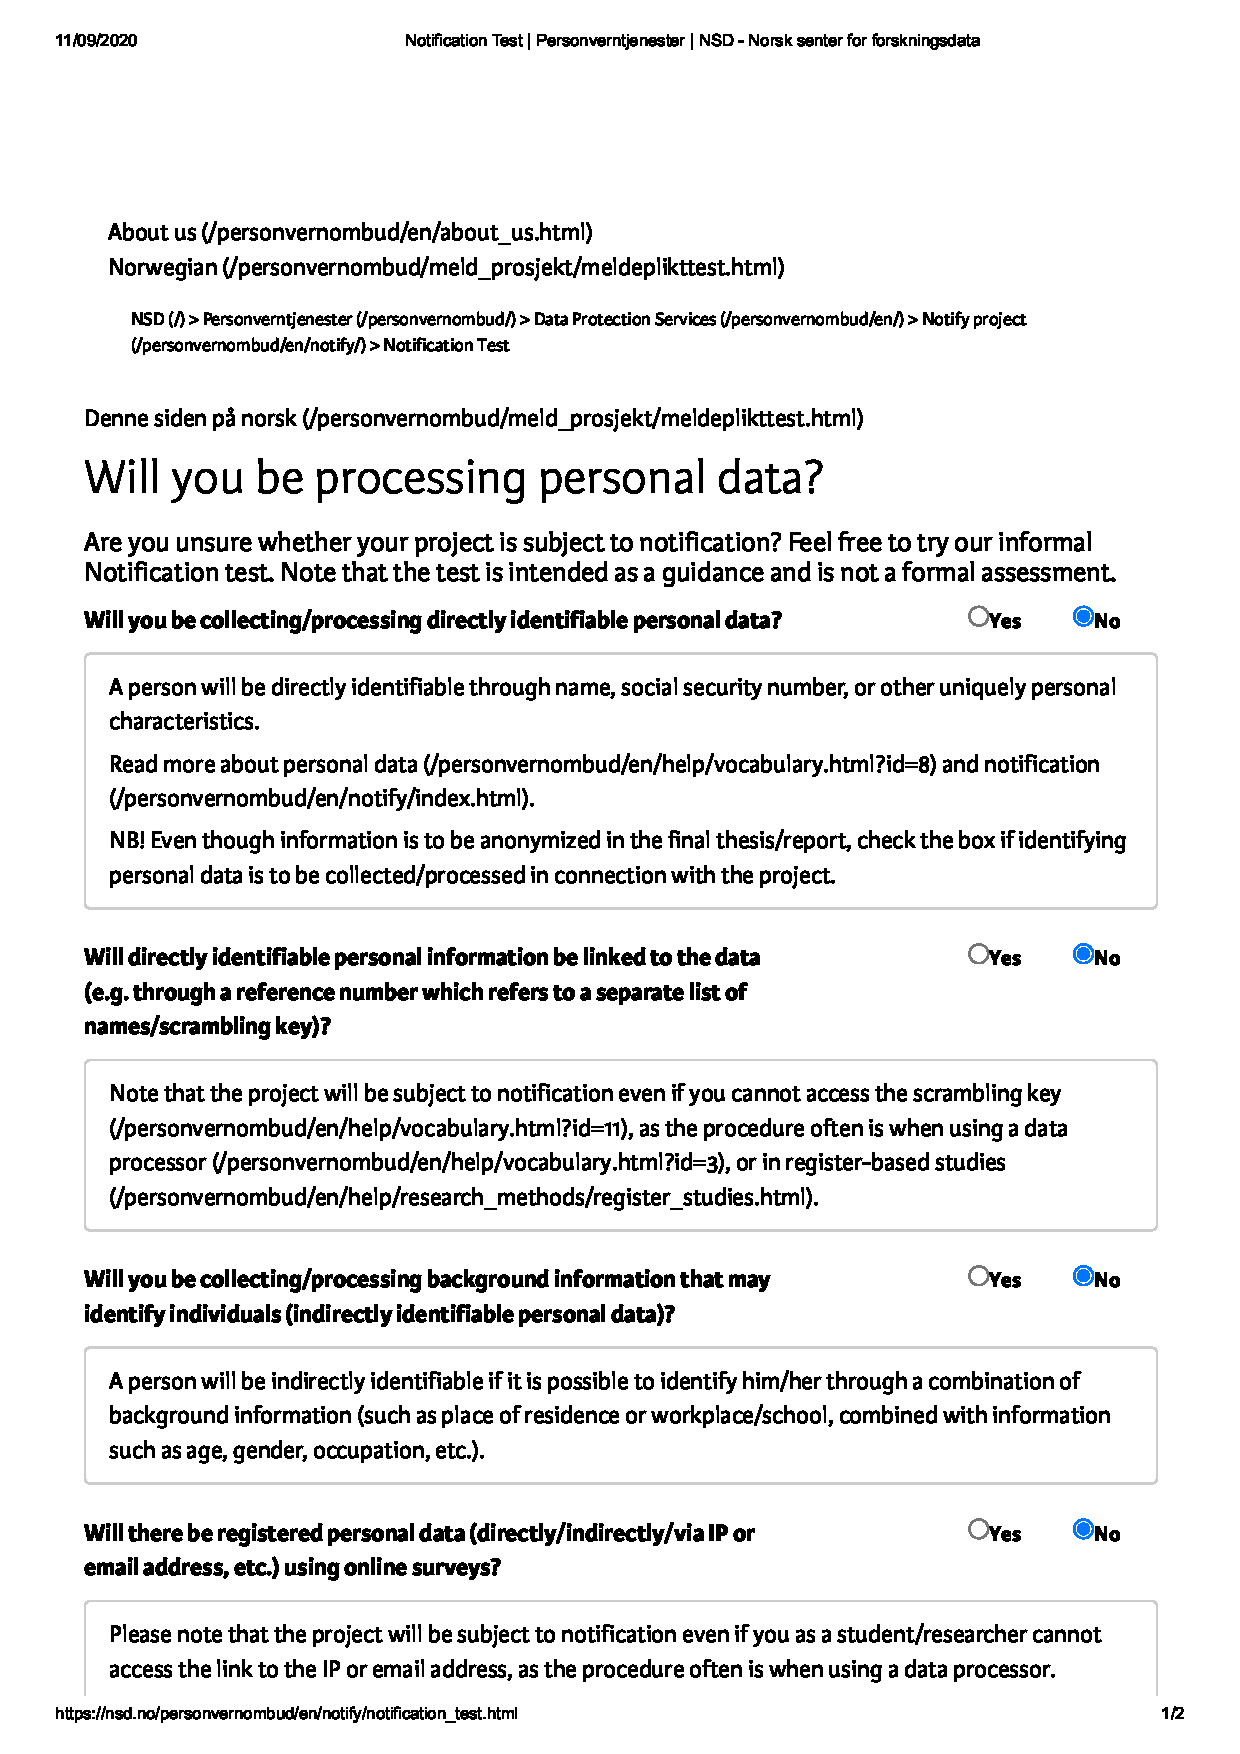
\includepdf[pages=-,fitpaper=true,noautoscale=true]{Appendices/Notification-Test.pdf}

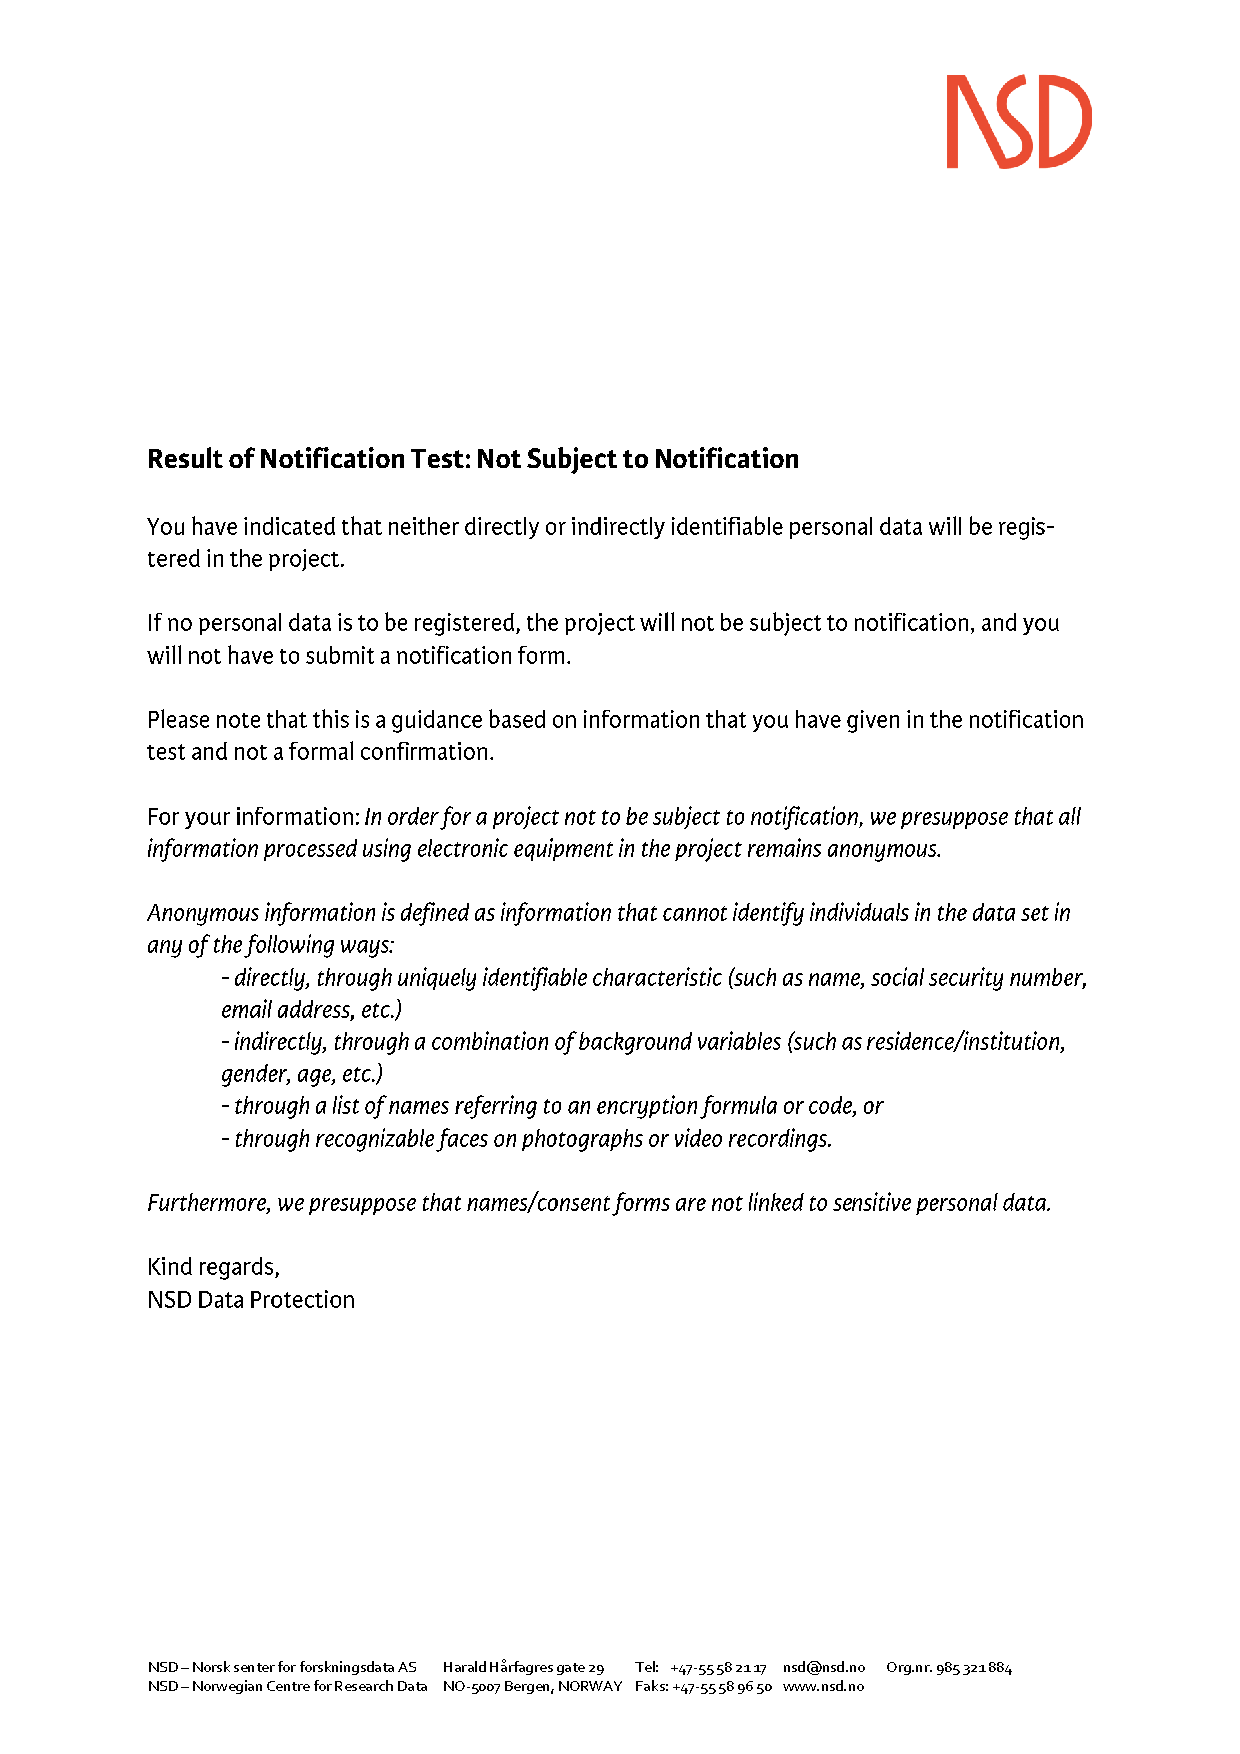
\includepdf[pages=-,fitpaper=true,noautoscale=true]{Appendices/not_subject_to_notification.pdf}


\section{Analysis Code, Additional Tables and Figures}

Full analysis code can be obtained from the author's GitHub page:

\href{https://github.com/tonyctan/CEMO-master-thesis}{https://github.com/tonyctan/CEMO-master-thesis}

\subsection{Data Merging}\label{R.reimport}

\begin{MAEcode}
    \lstinputlisting[language=R,style=vscodeR,linerange={5-114}]{./R/3 Reimport.R}
\end{MAEcode}

\MAEltable{tab:sample}{Summary of Participating Countries}{
      \begin{tabular}{ccl c rr c rr c rr}
      \toprule
      Country & Country & \multicolumn{1}{c}{Country} &       & \multicolumn{2}{c}{School} &       & \multicolumn{2}{c}{Student} &       & \multicolumn{2}{c}{Male} \\
      \cmidrule{5-6}\cmidrule{8-9}\cmidrule{11-12} ID  & code & \multicolumn{1}{c}{name} &       & \multicolumn{1}{c}{$n$} & \multicolumn{1}{c}{\%} &       & \multicolumn{1}{c}{$n$} & \multicolumn{1}{c}{\%} &       & \multicolumn{1}{c}{$n$} & \multicolumn{1}{c}{\%} \\
      \midrule
      76    & BRA   & Brazil &       & 595   & 8.97 &       & 8,310  & 7.75 &       & 4,045  & 48.68 \\
      100   & BGR   & Bulgaria &       & 197   & 2.97 &       & 4,110  & 3.84 &       & 2,147  & 52.24 \\
      124   & CAN   & Canada &       & 492   & 7.42 &       & 7,762  & 7.24 &       & 3,858  & 49.70 \\
      152   & CHL   & Chile &       & 251   & 3.79 &       & 4,482  & 4.18 &       & 2,254  & 50.29 \\
      233   & EST   & Estonia &       & 229   & 3.45 &       & 4,166  & 3.89 &       & 2,080  & 49.93 \\
      246   & FIN   & Finland &       & 204   & 3.08 &       & 4,328  & 4.04 &       & 2,199  & 50.81 \\
      268   & GEO   & Georgia &       & 319   & 4.81 &       & 4,320  & 4.03 &       & 2,239  & 51.83 \\
      360   & IND   & Indonesia &       & 395   & 5.96 &       & 7,132  & 6.66 &       & 3,454  & 48.43 \\
      380   & ITA   & Italy &       & 539   & 8.13 &       & 9,182  & 8.57 &       & 4,706  & 51.25 \\
      428   & LVA   & Latvia &       & 307   & 4.63 &       & 3,151  & 2.94 &       & 1,587  & 50.36 \\
      440   & LTU   & Lithuania &       & 349   & 5.26 &       & 4,075  & 3.80 &       & 2,060  & 50.55 \\
      528   & NLD   & The Netherlands &       & 151   & 2.28 &       & 3,042  & 2.84 &       & 1,549  & 50.92 \\
      604   & PER   & Peru &       & 337   & 5.08 &       & 4,732  & 4.42 &       & 2,390  & 50.51 \\
      616   & POL   & Poland &       & 235   & 3.54 &       & 4,294  & 4.01 &       & 2,080  & 48.44 \\
      620   & PRT   & Portugal &       & 276   & 4.16 &       & 4,568  & 4.26 &       & 2,320  & 50.79 \\
      643   & RUS   & Russian Federation &       & 558   & 8.42 &       & 9,124  & 8.51 &       & 4,601  & 50.43 \\
      688   & SRB   & Serbia &       & 186   & 2.81 &       & 3,874  & 3.62 &       & 1,951  & 50.36 \\
      703   & SVK   & Slovak Republic &       & 357   & 5.38 &       & 3,411  & 3.18 &       & 1,683  & 49.34 \\
      724   & ESP   & Spain &       & 491   & 7.40 &       & 9,361  & 8.74 &       & 4,695  & 50.15 \\
      840   & USA   & The USA &       & 163   & 2.46 &       & 3,738  & 3.49 &       & 1,871  & 50.05 \\
      \bottomrule
            &       & \multicolumn{1}{r}{Total} &       & 6,631  & 100 &       & 107,162 & 100 &       & 53,769 & 50.18 \\
      &&&&&&&&&&&\\
%      \cmidrule{5-12}
      \multicolumn{3}{r}{$\chi^2$ goodness-of-fit test} && \multicolumn{2}{c}{School} &       & \multicolumn{2}{c}{Student} &       & \multicolumn{2}{c}{Male} \\
      \cmidrule{5-6}\cmidrule{8-9}\cmidrule{11-12}
      &&&& $\chi^2_{19}$ & $p$ && $\chi^2_{19}$ & $p$ && $\chi^2_{19}$ & $p$\\
      \cmidrule{5-12}
      &&&& 1,105.8 & $<.001$ && 16,984 & $<.001$ && 20.9 & $.34$\\
%      \cmidrule{5-12}
      \end{tabular}
}{Twelve observations with missing school weights were removed. $\chi^2$ goodness-of-fit tests revealed that the data set was balanced in sex, but not all countries contributed equally to school and student counts.}

\ltable{tab:cronbach}{Scale Reliabilities (Cronbach's alphas) and Item Parameter References for Derived Variables based on IRT Scaling}{
    \begin{tabular}{ccl c@{\hskip 1cm} cccc c@{\hskip 1cm} c}
    \toprule
    Country & Country & \multicolumn{1}{c}{Country} &       & \multicolumn{4}{c}{School climate variable} &       & \multicolumn{1}{c}{Financial literacy} \\
\cmidrule{5-8}\cmidrule{10-10}    ID    & code  & \multicolumn{1}{c}{name} &       & \texttt{FLSCHOOL} & \texttt{FLFAMILY} & \texttt{NOBULLY} & \texttt{EDUSHORT} &       & \texttt{FLCONFIN} \\
    \midrule
    76    & BRA   & Brazil &       & .896 & .871 & .794 & .858 &       & .929 \\
    100   & BGR   & Bulgaria &       & .912 & .836 & .851 & .814 &       & .927 \\
    124   & CAN   & Canada &       & .904 & .856 & .758 & .816 &       & .900 \\
    152   & CHL   & Chile &       & .885 & .851 & .784 & .818 &       & .915 \\
    233   & EST   & Estonia &       & .865 & .833 & .709 & .752 &       & .872 \\
    246   & FIN   & Finland &       & .883 & .819 & .760 & .783 &       & .896 \\
    268   & GEO   & Georgia &       & .891 & .834 & .846 & .862 &       & .920 \\
    360   & IND   & Indonesia &       & .878 & .827 & .756 & .892 &       & .931 \\
    380   & ITA   & Italy &       & .857 & .798 & .795 & .840 &       & .898 \\
    428   & LVA   & Latvia &       & .846 & .813 & .703 & .780 &       & .897 \\
    440   & LTU   & Lithuania &       & .909 & .869 & .846 & .779 &       & .921 \\
    528   & NLD   & The Netherlands &       & .849 & .792 & .638 & .792 &       & .874 \\
    604   & PER   & Peru  &       & .847 & .813 & .758 & .882 &       & .903 \\
    616   & POL   & Poland &       & .878 & .830 & .771 & .839 &       & .913 \\
    620   & PRT   & Portugal &       & .896 & .844 & .775 & .849 &       & .899 \\
    643   & RUS   & Russian Federation &       & .892 & .855 & .726 & .874 &       & .911 \\
    688   & SRB   & Serbia &       & .926 & .853 & .838 & .786 &       & .939 \\
    703   & SVK   & Slovak Republic &       & .874 & .829 & .783 & .799 &       & .907 \\
    724   & ESP   & Spain &       & .879 & .812 & .779 & .854 &       & .912 \\
    840   & USA   & The USA &       & .908 & .839 & .756 & .881 &       & .909 \\
    \midrule
    \multicolumn{2}{l}{Reference for} & \multicolumn{1}{l}{OECD countries} & & \textsf{16.89} & \textsf{16.89} & \textsf{16.58} & \textsf{16.63} &       & \textsf{16.89} \\
    \multicolumn{2}{l}{scale reliabilities$\ ^\text{a}$} & \multicolumn{1}{l}{Partner countries} & & \textsf{16.90} & \textsf{16.90} & \textsf{16.59} & \textsf{16.64} &       & \textsf{16.90} \\
    &&&&&&&&&\\
    \multicolumn{3}{l}{Reference for item parameters$\ ^\text{b}$} & & \textsf{16.93} & \textsf{16.94} & \textsf{16.61} & \textsf{16.66} & & \textsf{16.91}\\
    \bottomrule
    \end{tabular}
}{$^\text{a}\ ^\text{b}$ Worksheet names in the associated \href{https://www.oecd.org/pisa/data/pisa2018technicalreport/PISA2018_Technical_Report_chapter-16_Background_Questionnaires.xlsx}{Excel file} accompanying Chapter 16 of \textit{PISA 2018 Technical Report} \parencite{PISAtech}.}{3}


\subsection{Multilevel Multiple Imputation}

\subsubsection{Mplus Input}\label{sec:MMI}

\begin{MAEcode}
    \lstinputlisting[style=vscodeMplus]{./Mplus/MMI/MMI.inp}
\end{MAEcode}

\subsubsection{Selected Mplus Output}

\begin{MAEcode}
    \lstinputlisting[style=vscodeMplus_out,linerange={2909-2967}]{./Mplus/MMI/MMI.out}
\end{MAEcode}

% Table generated by Excel2LaTeX from sheet 'Sheet1'
\ltable{tab:MMI}{Summary of Diagnostic Plots of Multilevel Multiple Imputation}{
      \begin{tabular}{ccclrrccc}
\toprule
      Parameter & \multicolumn{1}{c}{Parameter} & Modelling & \multicolumn{1}{c}{Brief} & \multicolumn{1}{c}{Posterior} & \multicolumn{1}{c}{Posterior} & 95\% credibility & Chain & AR-free \\
      number & \multicolumn{1}{c}{label} & level & \multicolumn{1}{c}{description} & \multicolumn{1}{c}{mean} & \multicolumn{1}{c}{variance} & interval & converged & chains \\
\midrule
      1     & \texttt{MALE}  & Within & Whether participant is male & 0.502 &       & (0.499, 0.505) & Yes   & 4 \\
      2     & \texttt{IMMI1GEN} & Within & Whether participant migrated to this country & 0.029 &       & (0.028, 0.030) & Yes   & 4 \\
      3     & \texttt{IMMI2GEN} & Within & Whether their parent did & 0.042 &       & (0.041, 0.044) & Yes   & 4 \\
      4     & \texttt{ESCS}  & Within & Index of economic, social and cultural status & $-$0.241 &       & ($-$0.247, $-$0.234) & Yes   & 4 \\
      5     & \texttt{FCFMLRTY} & Within & Familiarity with concepts of finance & 7.049 &       & (7.015, 7.083) & Yes   & 4 \\
      6     & \texttt{FLCONFIN} & Within & Confidence about financial matters & $-$0.072 &       & ($-$0.079, $-$0.065) & Yes   & 4 \\
      7     & \texttt{FLSCHOOL} & Within & Financial education in school lessons & 0.018 &       & (0.011, 0.024) & Yes   & 4 \\
      8     & \texttt{NOBULLY} & Within & Participant's experience of being bullied (reverse) & $-$0.059 &       & ($-$0.067, $-$0.052) & Yes   & 4 \\
      9     & \texttt{FLFAMILY} & Within & Parental involvement in matters of financial literacy & 0.064 &       & (0.057, 0.070) & Yes   & 4 \\
            &       &       &       &       &       &       &       &  \\
      10    & \texttt{MALE}  & Within & Whether participant is male &       & 0.250 & (0.248, 0.252) & Yes   & 4 \\
      11    & \texttt{IMMI1GEN} & Within & Whether participant migrated to this country &       & 0.028 & (0.028, 0.028) & Yes   & 4 \\
      12    & \texttt{IMMI2GEN} & Within & Whether their parent &       & 0.041 & (0.040, 0.041) & Yes   & 4 \\
      13    & \texttt{ESCS}  & Within & Index of economic, social and cultural status &       & 1.183 & (1.173, 1.193) & Yes   & 4 \\
      14    & \texttt{FCFMLRTY} & Within & Familiarity with concepts of finance &       & 29.754 & (29.495, 30.016) & Yes   & 4 \\
      15    & \texttt{FLCONFIN} & Within & Confidence about financial matters &       & 1.034 & (1.025, 1.044) & Yes   & 4 \\
      16    & \texttt{FLSCHOOL} & Within & Financial education in school lessons &       & 1.040 & (1.031, 1.049) & Yes   & 4 \\
      17    & \texttt{NOBULLY} & Within & Participant's experience of being bullied (reverse) &       & 1.111 & (1.100, 1.121) & Yes   & 4 \\
      18    & \texttt{FLFAMILY} & Within & Parental involvement in matters of financial literacy &       & 1.090 & (1.080, 1.100) & Yes   & 4 \\
            &       &       &       &       &       &       &       &  \\
      19    & \texttt{STRAIO} & Between & Student$-$teacher ratio & 13.873 &       & (13.607, 14.139) & Yes   & 4 \\
      20    & \texttt{EDUSHORT} & Between & Shortage of educational material & 0.131 &       & (0.106, 0.157) & Yes   & 4 \\
            &       &       &       &       &       &       &       &  \\
      21    & \texttt{STRAIO} & Between & Student$-$teacher ratio &       & 103.532 & (99.750, 107.430) & Yes   & 4 \\
      22    & \texttt{EDUSHORT} & Between & Shortage of educational material &       & 1.074 & (1.037, 1.112) & Yes   & 4 \\
\bottomrule
      \end{tabular}
}{Notes go here.}{6}

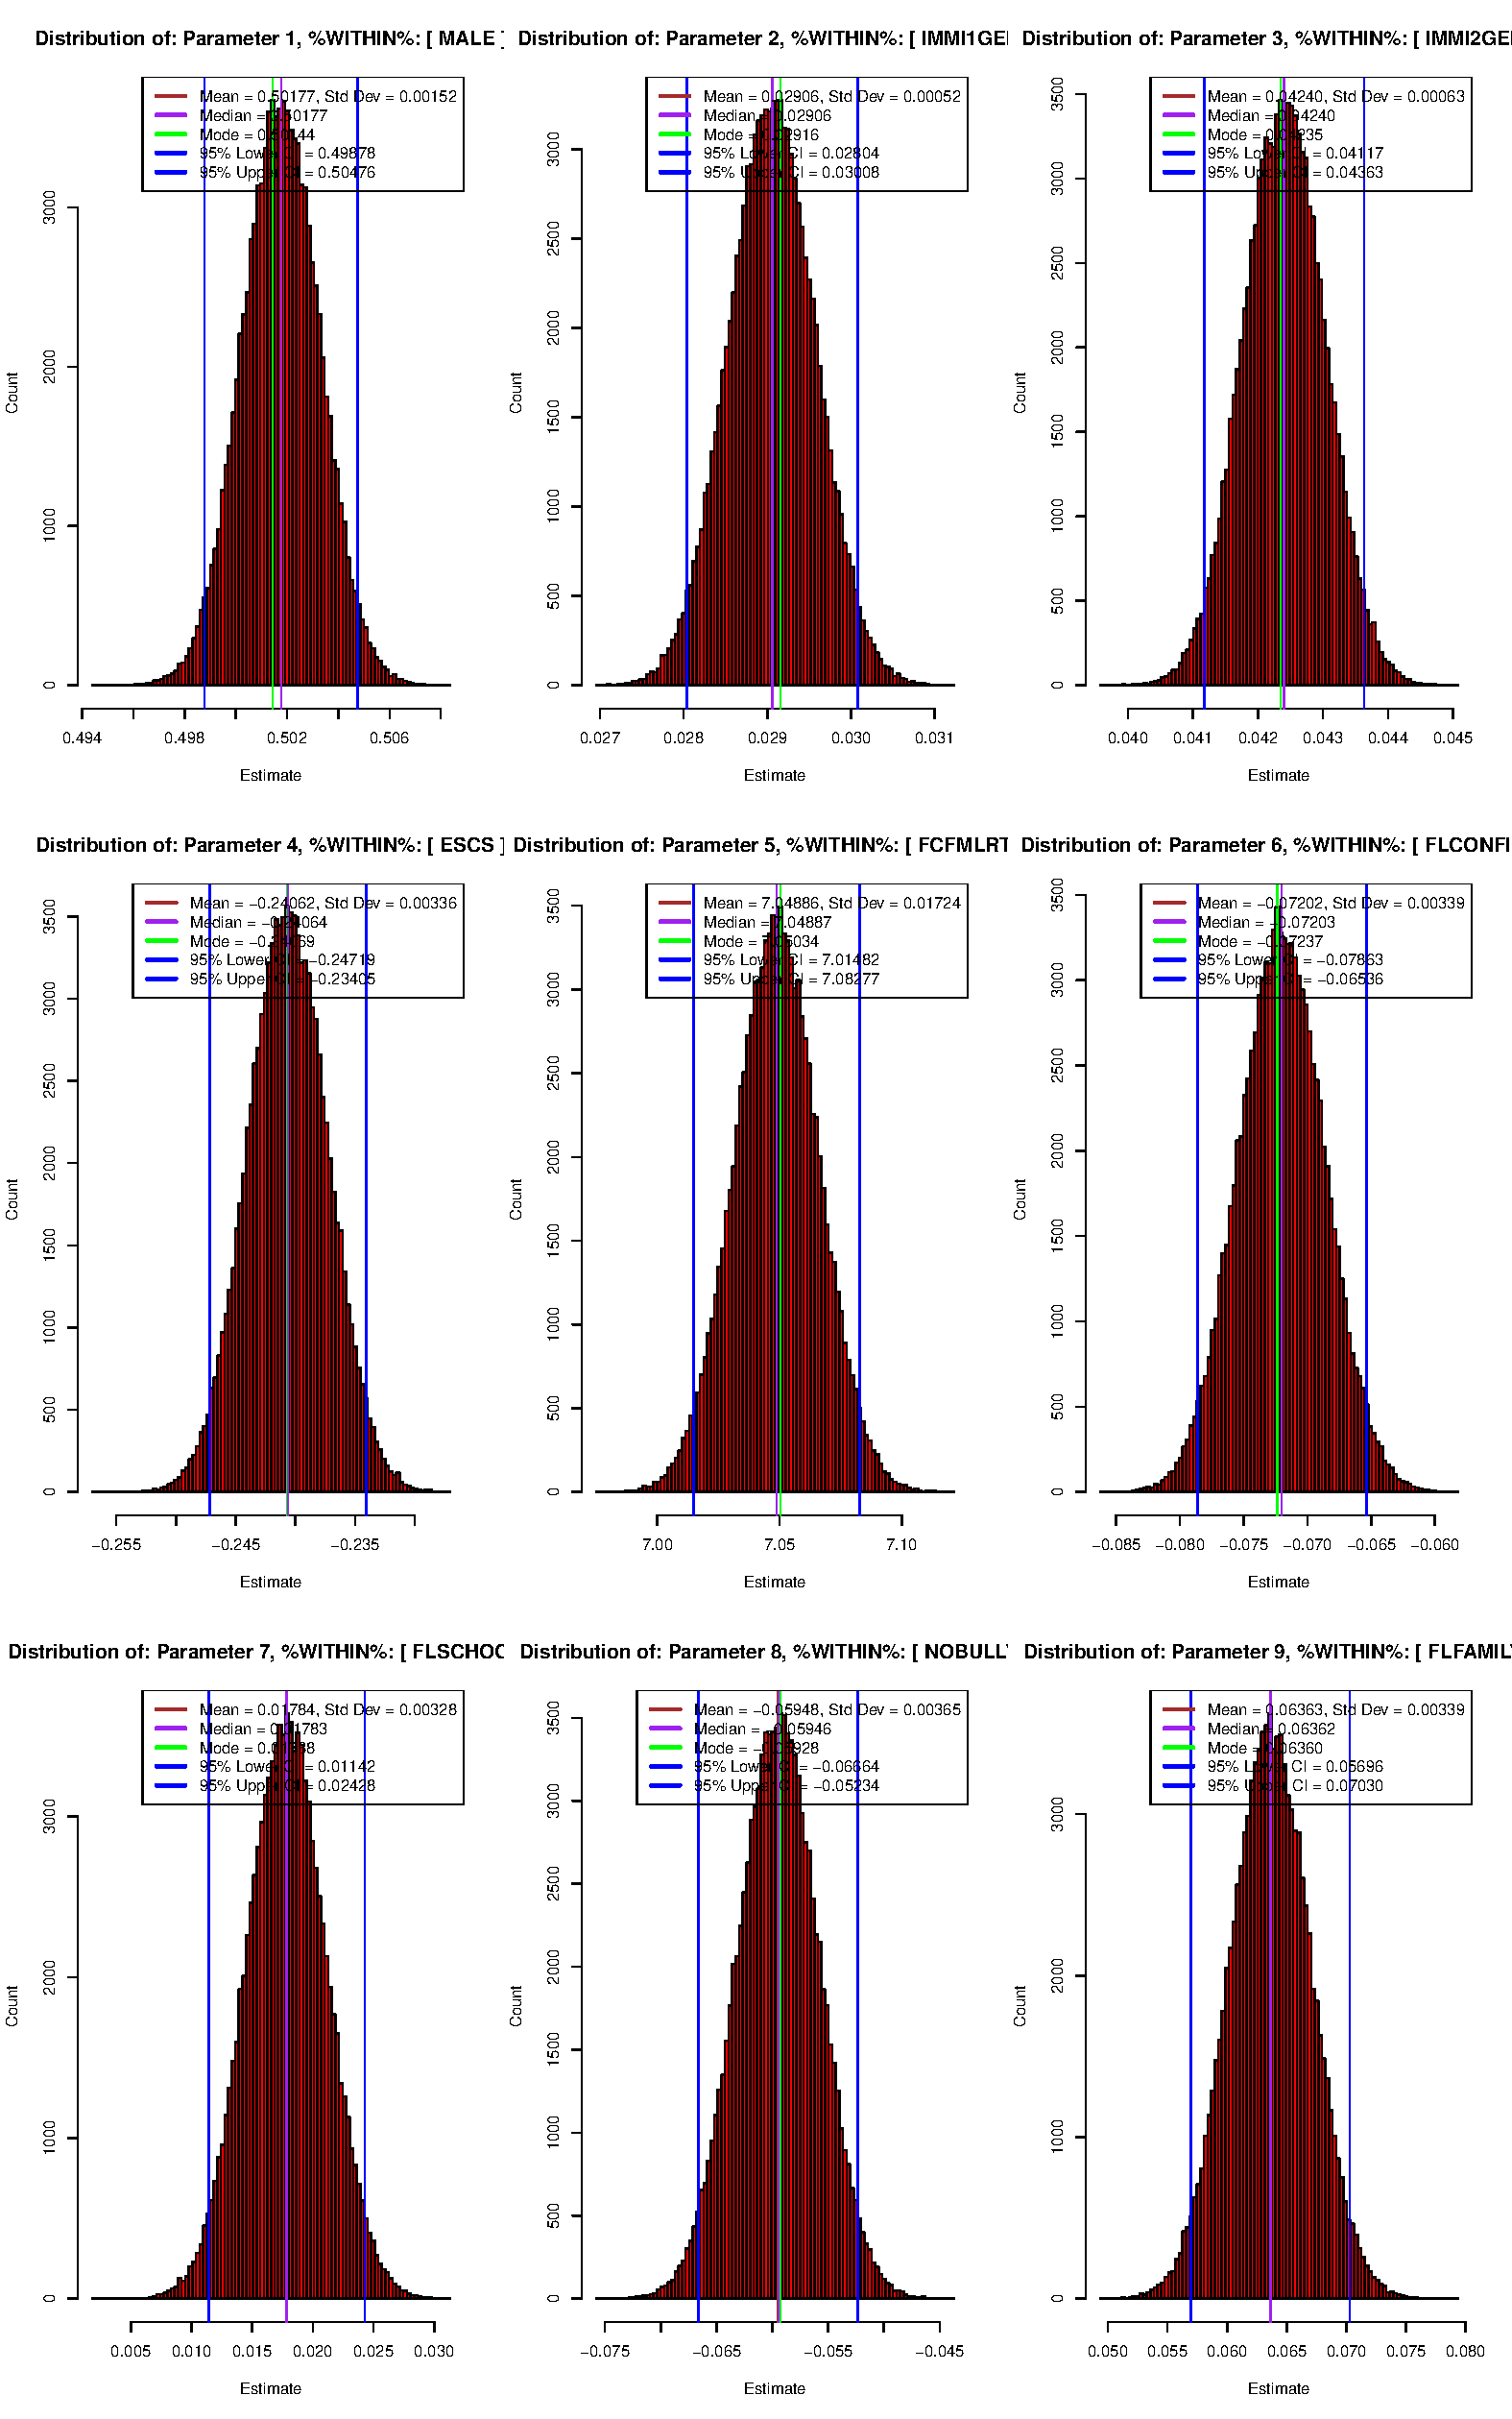
\includepdf[pages=-,width=\textwidth,pagecommand={}]{./Figures/MMI_diagnostic.pdf}

\subsection{MSEM Analysis Code}

\subsubsection{Mplus Input}

\begin{MAEcode}
    \lstinputlisting[style=vscodeMplus]{./Mplus/M3/Two-structured.inp}
\end{MAEcode}

\subsubsection{Selected Mplus Output}\label{sec:rsq}

\begin{MAEcode}
    \lstinputlisting[style=vscodeMplus_out,linerange={991-1007}]{./Mplus/M3/Two-structured.out}
\end{MAEcode}


\section{Stimuli, Test Items and Additional Materials}
\label{app:C}

\MAEindent

Include extra information here.

\end{document}
